\documentclass[11pt,fleqn]{book}
\usepackage[top=3cm,bottom=3cm,left=3.2cm,right=3.2cm,headsep=10pt,letterpaper]{geometry}
%中文支持
\usepackage[space]{ctex}
\usepackage[utf8]{inputenc}
\usepackage{amsmath}
\usepackage{amssymb}
\usepackage{times}
\usepackage{titlesec}
\usepackage[table]{xcolor}
%结构化
\graphicspath{{./figure/}}
\usepackage{subfiles}
\usepackage{blindtext}
\usepackage{listings}%设置C风格代码格式
\usepackage{csquotes}%设置引用风格
\usepackage{graphicx}
\usepackage{float}
\usepackage{pythonhighlight}
\usepackage{caption}
\usepackage{subfigure}
\usepackage{longtable}
\setlength{\arrayrulewidth}{0.5mm}
\usepackage{hyperref}
\usepackage{fancyhdr}
\pagestyle{fancy}
\fancyhf{}
\rhead{\rightmark}
\rfoot{\thepage}
\renewcommand{\headrulewidth}{2pt}%设置页眉标线
\renewcommand{\footrulewidth}{1pt}%设置页脚标线

\pagenumbering{arabic}
\hypersetup{
    colorlinks=true,
    linkcolor=blue,
    filecolor=magenta,      
    urlcolor=cyan,
}
\urlstyle{same}
%字体设置
%\usepackage{times} % Use the Times font for headings
\usepackage{mathptmx} % Use the Adobe Times Roman as the default text font together with math symbols from the Sym­bol, Chancery and 
%tktz画图
\usepackage{tkz-graph}
\GraphInit[vstyle = Shade]
\tikzset{
  LabelStyle/.style = { rectangle, rounded corners, draw,
                        minimum width = 2em, fill = green!50,
                        text = red, font = \bfseries },
  VertexStyle/.append style = { inner sep=5pt,
                                font = \Large\bfseries},
  EdgeStyle/.append style = {->, bend left} }

\begin{document}
\frontmatter
\tableofcontents % Print the table of contents itself
\mainmatter
\definecolor{codegreen}{rgb}{0,0.6,0}
\definecolor{codegray}{rgb}{0.5,0.5,0.5}
\definecolor{codepurple}{rgb}{0.58,0,0.82}
\definecolor{backcolour}{rgb}{0.95,0.95,0.92}
 
\lstdefinestyle{mystyle}{
    backgroundcolor=\color{backcolour},   
    commentstyle=\color{codegreen},
    keywordstyle=\color{magenta},
    numberstyle=\tiny\color{codegray},
    stringstyle=\color{codepurple},
    basicstyle=\footnotesize,
    breakatwhitespace=false,         
    breaklines=true,                 
    captionpos=b,                    
    keepspaces=true,                 
    numbers=left,                    
    numbersep=5pt,                  
    showspaces=false,                
    showstringspaces=false,
    showtabs=false,                  
    tabsize=2
}
 
\lstset{style=mystyle}
\section{移动平台}
TensorFlow对于移动平台被设计为一个好的深度学习解决方案。
当前我们已经有两个解决方案用于部署机器学习应用到移动设备和嵌入式设备:\href{https://www.tensorflow.org/mobile/mobile_intro?hl=zh-cn}{TensorFlow for Mobile}和\href{https://www.tensorflow.org/mobile/tflite/index?hl=zh-cn}{TensorFlow Lite}。
\subsection{TensorFlow LiteVS TensorFlow Mobile}
下面是两者的一些不同之处:
\begin{itemize}
\item TensorFlow Lite是TensorFlow Mobile的一个进化版本。在多属性框虾,用TensorFlow Lite开发的app二进制文件更小,依赖更小,性能更强。
\item TensorFlow Lite是在开发者预览中,因此不是所有情况都能覆盖。我们希望你用TensorFlow Mobile覆盖产品。
\item TensorFlow Lite仅仅支持有限的操作,因此不是所有的模型都能在上面运行的很好。TensorFlow Mobile对函数有一个更完整的支持。
\end{itemize}
TensorFlow Lite为移动平台提供了更好的性能和更小的文件尺寸如果在它们的平台上一些硬件加速功能加速功能可以使用的话。另外,它有更少的依赖以至于它可能被构建运行在更简单的,资源首先得设备上。TensorFlow Lite可允许通过\href{https://developer.android.com/ndk/guides/neuralnetworks/index.html?hl=zh-cn}{Neural Networks API}加速。

TensorFlow Lite当前已经覆盖了有限的一些操作。尽管默认TensorFlow Mobile支持仅仅支持有限的操作,原则上如果你用TensorFlow的任意操作,它能被自定义构建kernel。这样用不支持TensorFlow Lite的情况将继续支持TensorFlow Mobile。正如TensorFlow Lite设计的,它将添加额外的操作,将被很容易决定。
\subsection{介绍TensorFlow Lite}
TensorFlow Lite是针对移动设备和嵌入式设备的TensorFlow的轻量级的解决方案。他以很低的代价和小的二进制文件尺寸在设备上进行机器学习推理。TensorFlow Lite也支持用\href{https://developer.android.com/ndk/guides/neuralnetworks/index.html?hl=zh-cn}{Android Neural Networks API}进行加速。

TensorFlow Lite用一些想优化移动app核心,预先融合激活,量化内核的技术获取更低的消耗获得更小更快的模型。
大多数的TensorFlow Lite文档在\href{https://github.com/tensorflow/tensorflow/tree/master/tensorflow/contrib/lite}{Github}上。
\subsection{TensorFlow Lite包含什么?}
TensorFlow Lite包含一系列核心操作,包括针对移动平台调整的量化和浮点。他么通过预先融合激活和偏置加强性能和量化精度。另外,TensorFlow Lite也支持在模型中使用自定义的操作。
\section{介绍TensorFlow Mobile}
TensorFLow被设计成为在想Android和iOS的移动平台上的一个好的深度学习解决方案。移动想到应该帮助你理解机器学习可以在移动平台上工作以及如何高效整合TensorFlow到你的移动app中。
\subsection{关于这个向导}
这个向导的是已经有一个能在桌面环境下工作的模型想整合模型进入移动应用中,不能用TensorFlow Lite,下面是你将面对的主要挑战:
\begin{itemize}
    \item 明白如何使用TensorFlow for mobile 
    \item 为你的平台构建TensorFlow
    \item 整合TensorFlow库进你的应用
    \item 为你的移动部署准备你的模型文件
    \item 优化时延,RAM使用,模型文件大小,二进制文件大小
\end{itemize}
\subsection{常用的机器学习情景}
\textbf{为什么在移动设备上运行TensorFlow?}\newline
创痛的深度学习结合数据中心和大型的高性能GPU集群。然而,通过网络连接发送设备数据这可能很昂贵耗费时间。运行在移动设备上是可能的当你继续不可能必须等待网络处理传送每个交互。下面是在设备上运行深度学习的常见情景。
\subsection{语音识别}
一些有趣的应用可能构建在一个语义驱动的借口上,这些请求在设备上处理。很多时候永不没有给任何指令,持续和远程服务器通信将浪费带宽,因为很多情况下很安静或者有背景噪声。为了解决这个问题一个常见的通常是运行一个晓得神经网络在设备上\href{https://www.tensorflow.org/tutorials/audio_recognition?hl=zh-cn}{ listening out for a particular keyword}当关键字被发现,一些剩下的场景可能是如果需要更多的计算力则发送给服务器进一步处理。
\subsection{图像识别}
对于移动app理解摄像头场景是很有用的。如果你的用户拍摄了照片,识别他们可能帮助你的相机app更好的过滤或者标记相片以至于他们能轻松地找到。这对于嵌入式应用来说也是很重要的,因此你可以用图像传感器检测一些感兴趣的条件,是否并未动物在野生环境下或者\href{https://svds.com/tensorflow-image-recognition-raspberry-pi/}{报告你的训练运行多晚}
TensorFlow结合一些云连号的目标识别的模型,他们可以运行在你的移动设备上。你可以尝试\href{https://codelabs.developers.google.com/codelabs/tensorflow-for-poets/index.html?hl=zh-cn#0}{ Tensorflow for Poets }和\href{https://codelabs.developers.google.com/codelabs/tensorflow-for-poets-2/index.html?hl=zh-cn#0}{Tensorflow for Poets 2: Optimize for Mobile }代码实验室查看如何获取已经训练好的模型运行非常快,轻量级的训练叫它识别特殊物体,优化他在手机端的运行。
\subsection{对象定位}
有是有知道对象在图像中的位置和对象是什么一样重要一些参数使用情景可能从一个移动app获益,比如说指导用户到正确的组件提供帮组修复他们的无线网络或者在一些特殊的场景提供信息覆盖其上。嵌入式应用经常需要计数传给他们的对象,是否宠物在庄稼地里或者人,汽车,自行车将通过街道信号灯。
TensorFlow提供一个预先训练好的模型标描绘在图像中检测到的人一个框,结合追踪代码实时跟踪他们。最终对于你尝试统计多少对象被实时呈现是很重要的,因此放一个新的对象进入或者离开场景时他给你一个好的想法。对于Android设备我们给了一个可用的代码在\href{https://github.com/tensorflow/tensorflow/tree/master/tensorflow/examples/android}{Github},更多以\href{https://github.com/tensorflow/models/tree/master/object_detection/README.md}{常用的对象检测模型}也可用
\subsection{手势识别}
不论是用手或者其他的姿势控制应用,从图像中识别或者分析加速度传感器数据是很有用的。创建这些模型超过了这个向导的内容,但是TensorFlow能高效的部署他们。
\subsection{光学字符识别}
Google翻译的实时相机查看是一个设备检测文字的交互高效的好的例子。在图像中识别文字有一些步骤,首先识别文字呈现的区域,就是目标定位,可以使用类似的技术解决。当你有文字区域后你将需要解释他为字符,然后用语言模型猜测他们表达的是什么意思。最简单的评估文字表达的意思是分割文本行为单个的文字然后使用简单的神经网络框住每个字符。你可以用MNIST模型(TensorFlow导航)获得一个好的结果,尽管尼克徐想一个更高的解决输入。一个高级的使用是用LSTM模型处理一行文本,模型自己处理片段为不同的字符,
\subsection{翻译}
即使在没有网络的情况下准确的翻译一种语言到另一种语言是很重要的使用场景。深度网络在这些任务上很高效,你能找到一些不同的文学模型描述。经常seq2seq循环模型能运行单个图处理整个翻译,结合需要运行分割的解析场景。
\subsection{文本分类}
如果你想在用户输入和阅读的基础上给出相关的建议,理解文本的意思将变得很有用文本分类是一个伞包含了从拘役分析到组提发现。你可能有自己想应用的策略或者标签,因此最好的地方是开始一个想\href{https://github.com/tensorflow/models/tree/master/skip_thoughts/}{Skip-Thoughts}然后在你自己的例子上训练。
\subsection{{语音合成}
语音合成可能是一个好的方法给予用户返回或者帮助,最近的想\href{https://deepmind.com/blog/wavenet-generative-model-raw-audio/}{WaveNet}}显示了深度学习可以提供非常自然的声音。
\subsection{移动机器学习和云}
一些使用场景的例子在设备网络结合云服务上给出一个想法。云在控制的环境中有强大的计算力,但是运行在设备山更可以提供更高效的交互。在这种情况下云是不可用的或者你的云能力首先,你可以提供一个离线的试验或者通过在设备上处理减少云负载。
在设备上计算也是一个信号当他的时间交换了云上的工作。一个好的例子是语音中的关键词检测,因为设备能直接听关键词,一旦识别然后触发了一些通信和基于云的语音识别。没有在设备上的组件,整个应用将不可用,这些样本存在通过一些其他的应用识别一些sensor的输入对于更进一步的处理以创建一些有趣的产品是足够感兴趣的。
\subsection{你应该拥有什么软件和硬件?}
TensorFlow运行在Ubuntu,Windows10,OS X上。详细的所有支持的操作系统和安装说明查看\href{https://www.tensorflow.org/install/index?hl=zh-cn}{Installing tensorFlow}
注意我们为移动TensorFlow提供多个事例代码要求你从源代码编译TensorFlow,因此你将需要pip install在示例代码上工作。为了试验移动例子,你将需要一个设备用于开发,用\href{https://developer.android.com/studio/install.html?hl=zh-cn}{Android Studio}如果你开发iOS使用\href{https://developer.apple.com/xcode/}{XCode}
\subsection{在开始之前你需要做什么?}
首先思考如何获得移动机器学习解决方案。
\begin{enumerate}
    \item 确定你的问题是否能通过移动机器学习解决
    \item 创建标记的数据集定义你的问题
    \item 为你的问题选择高效的模型
\end{enumerate}
\subsection{你的问题是否是移动机器学习能解决的?}
关于你想解决的问题当你有一个想法时,你需要计划如何构建你的解。最重要的一步是确保你的问题实际上是可解的,最好的方法是用人力循环测试。
例如如果你想用语音驱动机器人玩具车。尝试从设备记录一些声音,监听如果你可以理解说了什么返回它。经常你将在捕获处理上找到一些问题,像电机淹没了声音或者因为距离不能被听到,你应该在模型处理调查钱处理这些问题。
另一个例子是给一张冲你的app拍的照片给人看看是否人能分辨他们是什么。用这种方法寻找。如果他们不能左到(例如尝试从照片估计食物的热量也许是不可能的应为所有的白色的汤都是一样的,然后你将重新设计你的试验处理它。)一个好的原则是如果一个人不能处理这个任务,训练机器人左到更好是很困难的。
\subsection{创建标记的数据集}
在你解决了一些基本的问题后,你需要创建一个标记的数据集来定义你尝试解决的问题。这一步是极其重要的,甚至比选择使用的模型还要重要。你想他能作为你的实际场景下的表达,因此模型将在你教他的任务下变得高效。调查工具尽可能高效和精确地标记数据也是很有价值的。例如,如果你能转化在web接口的点击为键盘上的快捷键,你也许能加速生成过程。你应该自己初始化标记,因此你可以了解他的难度和可能的错误,可能改变你的标记和数据部或处理来避免他。当你和你的团队能组合标记样本(对多数的样本生成相同的标签表示赞同),你可以尝试捕获你的只是在一个手册相互交流而不是如何运行相同的过程。
\subsection{选择一个高效的模型}
下一步是选择一个高效的模型使用。如果有人已经实现了和你的模型类似的你需要的模型你也许能避免训练一个模型;我们在Github上有一个\href{https://github.com/tensorflow/models}{模型仓库},学习你能找到的最简单的模型,尝试在当你有一个小的标记数据是开始,因此你当你能快速迭代时将获得最好的结果。很多的时间花费在训练一个模型和在真是应用上运行上,更好的结果你将在最终看到。通常一个算的获得很高的训练精度但是对于实际应用却没有用因为数据集和真是使用上不匹配。端到端样本使用尽可能创建一个始终如一的用户体验。
\subsection{下一步}
我么你建议你从我们给的\href{https://www.tensorflow.org/mobile/android_build?hl=zh-cn}{Android}和\href{https://www.tensorflow.org/mobile/ios_build?hl=zh-cn}{iOS} demo中开始。
TensorFlow Lite定义了一个新的基于\href{https://google.github.io/flatbuffers/}{FlatBuffers}模型文件格式。FlatBuffers是一个开源,高效,跨平台的序列化库。类似\href{https://developers.google.com/protocol-buffers/?hl=en}{Protocol buffers},但是主要的不同是在访问数据时FlatBuffers不需要解析/解包步骤为一个二次表达,经常和对象内存分配成对出现。FlatBuffers代码足迹比protocal buffers更小。

TensorFlow Lite是一个新的移动量化平台目标是跟中app的负载和速度。解释器用一个静态图和一个自定义的(少量动态)内存分配器企鹅报最小的砸入,初始化,和高效执行。

TensorFlow Lite 提供一个接口用于硬件加速,如果硬件加速在设备上可用。它通过Android Neural Network库(Android O-MR1)加速。
\subsection{为什么需要一个新的专为移动平台设计的库?}
机器学习正在改变计算范式,我们看到了嵌入式平台和移动平台融合的趋势。用户期望和他们的设备通过摄像头,声音交互模型以自然,人类喜欢的方式交互。
下面是融合的一些因素:
\begin{itemize}
\item 在半导体硅上的创新是硬件加速的新的可能,想Android Neural Network API框架使得利用硬件加速成为可能
\item 现在先进的实时计算机视觉和语义理解一定导致移动优化基准模型正在被开源
\item 在设备智能上为广泛的智能应用创建了新的可能。
\item 对用户数据隐私不需要离开移动设备的兴趣
\item 服务离线情况,这里的设备不需要连接网络
\end{itemize}
我们相信下一波机器学习应用浪潮将来自于移动平台和嵌入式设备。
\subsection{TensorFlow Lite 开发者预览重点}
作为开发者预览的TensorFlow Lite包含如下内容:
\begin{itemize}
\item 包括量化的和浮点的核心操作已经被转化用于移动平台。这可能用于创建和运行自定义的模型。开发者可以在他们的模型中写自己的操作
\item 一个新的\href{https://google.github.io/flatbuffers/}{FlatBuffers}模型文件格式
\item 结合内和核心优化在移动设备上更快的执行
\item TensorFlow转化器转化TensorFlow-trained的模型为TensorFlow Lite格式
\item 更小的尺寸:TensorFlow Lite当所有的操作被连接小于300KB,当用操作徐娅支持Inception V3和MobileNet时小于200KB
\item 预先测试的模型:所有的模型被确保效果\begin{itemize}
\item Inception V3,一个流行在图像上的侦测对象的模型
\item \href{https://github.com/tensorflow/models/blob/master/research/slim/nets/mobilenet_v1.md}{MobileNets}当用于资源受限的设备或者谦如水应用的一个熟悉的针对移动平台的高效的最大化精确度计算机视觉模型。塔恩很小,低时延,低功耗模型参数化以范主各种资源受限的情况。他们能被构建用于分类,检测,嵌入和分割。MobileNet模型很小但是相比Inception V3\href{https://research.googleblog.com/2017/06/mobilenets-open-source-models-for.html}{精度低}
\item 在设备智能回复,在设备模型上对输入文本信息给出相关的建议信息回复。模型被构建用于内存有限的设备像手表和手机等设备上并且他对于第一方和第三方app已经被成功的用于\href{https://research.googleblog.com/2017/02/on-device-machine-intelligence.html}{Smart Replies onAndroid Wear}
\item 量化的MobileNet模型版本,运行比没有量化的版本在CPU上运行更快
\item 新的Android示例程序解释TensorFlow Lite结合量化的MobileNet模型用于目标检测是如何使用的
\item Java 和C++ API支持
\end{itemize}
\end{itemize}
\begin{quote}
这是一个开发者版本,可能子啊将来的API中修改,我们不能保证这个版本向后兼容
\end{quote}
\subsection{开始}
我们推荐你结合上面的预先测试好的模型进行尝试。如果你有一个存在的模型,你讲需要测试是否你的模型和转化器和支持的操作集合兼容。为了测试模型,查看\href{https://github.com/tensorflow/tensorflow/tree/master/tensorflow/contrib/lite}{documenttation on GitHub}
\subsection{重新训练Inception V3或者MobileNet用于用户自定义的数据集}
上面提到的模型是基于ImageNet数据集1000个分类的数据进行训练的。如果这些类对你的使用不相关或者没用,你将需要重新训练模型。这个技术成为迁移学习,在一个已经训练好的模型上重新训练一个类似的问题。深度学习训练可能花费很长时间,但是迁移学习能以被很快的使用。为了做这个事,你将需要生成你的自定义的数据集结合相关的类标记。

\href{https://codelabs.developers.google.com/codelabs/tensorflow-for-poets/?hl=zh-cn}{TensorFlow for Poets}代码实验室告诉你如何一步步左到。重新训练代码支持重新训练用于浮点和量化接口。
\subsection{TensorFlow Lite 架构}
下面的图显示了TensorFlow Lite的架构设计
\begin{figure}[H]
\centering
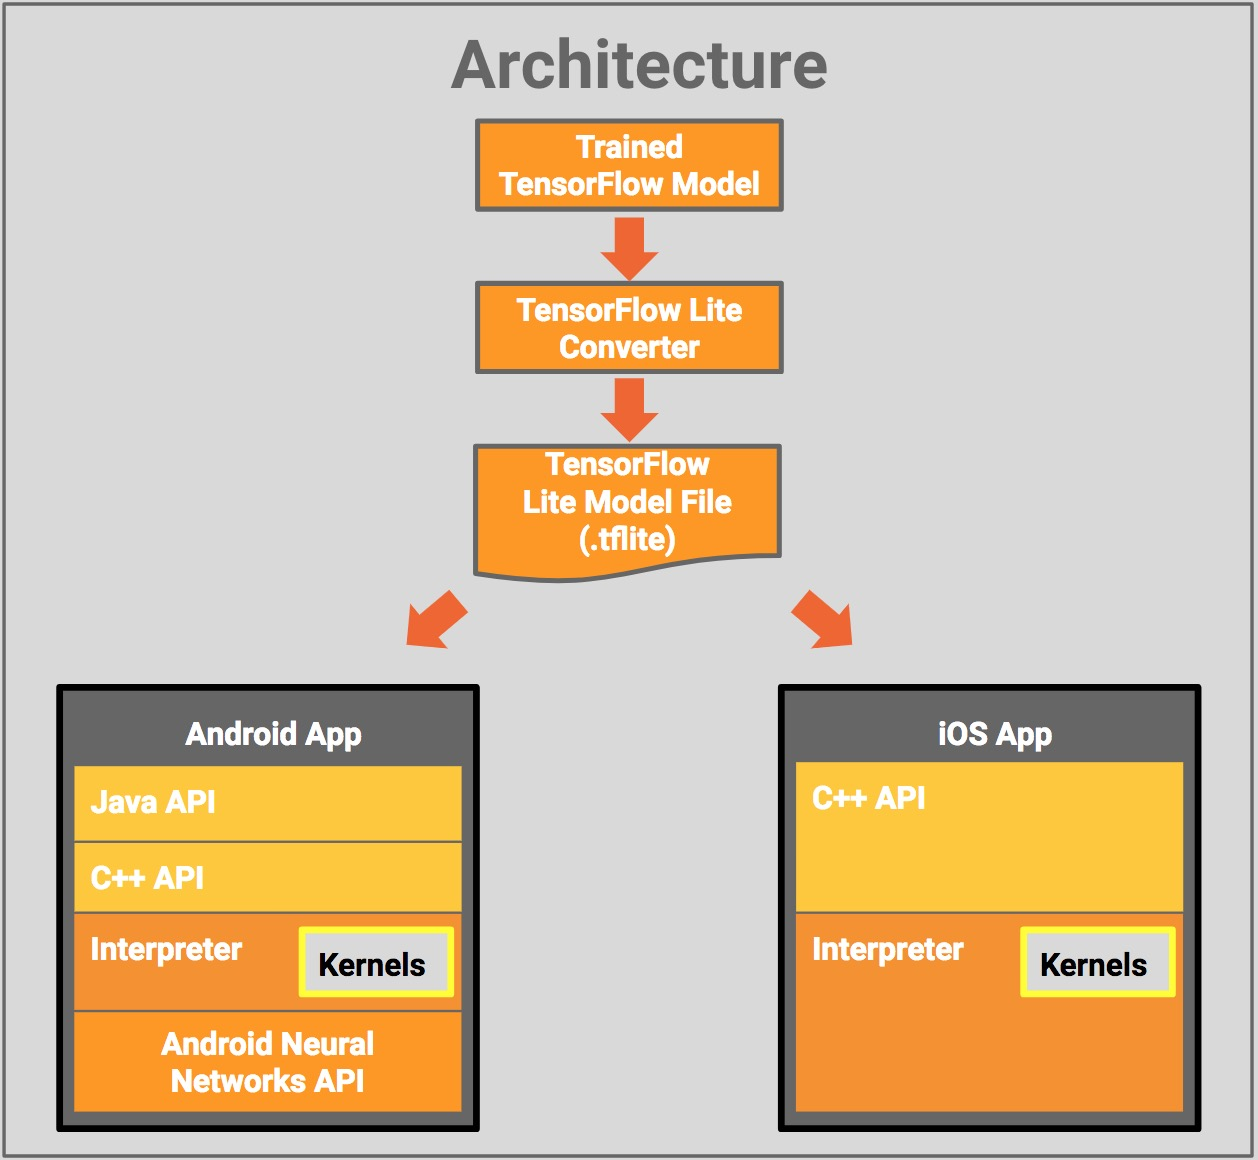
\includegraphics[scale=0.3]{tflite-architecture.jpg}
\caption{TensorFlow Lite 架构}
\end{figure}
在磁盘上开始一个训练的模型,你将用TensorFlow Lite转化器转化模型为TensorFlow Lite文件格式(.tflite)。然后你可以用转化的文件在你的移动应用上。
部署TensorFlow Lite模型文件:
\begin{itemize}
\item Java API:一个方便的在Android上围绕C++ API的包装器
\item C++ API:载入TEnsorFlow Lite模型文件,调用解释器,相同的库在Android和IOS上都可用
\item 解释器:用一些可信执行模型。解释器支持选择核心载入;没有核心仅仅100KB,3,全部载入核心300KB。这是从TensorFlow Mobile要求的1.5M重要的减小
\item 在选择的Android设备上,解释器讲用Android Neural Network API用于硬件加速,或者如果没有可用的默认使用CPU执行。
\end{itemize}
你可以用C++ API实现用于解释器的自定义核心。
\subsection{将来的工作}
在将来的版本中TensorFlow Lite讲支持更多的模型和内建操作,包括用于对固定点和浮点模型的运行改进,和让开发者更容易的开发工作刘和对其它更小的设备的支持等等。正如我们继续开发,我们希望TensorFlow Lite将简化开发者对于小型设备的开发者经历。

将来几哈用指定的机器学习硬件获取更好的可能性能用于类似设备上的类似模型。
\subsection{下一步}
对于开发者预览,多数文档在GitHub上。请查看\href{https://github.com/tensorflow/tensorflow/tree/master/tensorflow/contrib/lite}{TensorFlow Lite repository}获取更多信息和代码样例,事例应用和更多。

\section{在Android上构建TensorFlow}
为了在Android设备上开始TensorFlow,我们通过两种方法构建我们的TensorFlow移动demo部署在Android设备上。第一种是Android Studio,让你在IDE下构建和部署。第二个是在Bazel上构建通过ADB命令行部署。

为什么选择一个或者其他的方法?
一个简单的在Android设备上使用TensorFlow的方法是用Android Studio。如果你没有计划自定义你的TensorFlow构建或者你想用Android Studio的编辑器或者其他的特性去构建一个app仅仅想添加TensorFlow在其之上,我们推荐你使用Android Studio。

如果你正在使用自定义的操作或者有一些其他的原因构建TensorFlow,向下滚动鼠标查看\href{https://www.tensorflow.org/mobile/android_build?hl=zh-cn#build_the_demo_using_bazel} {building the demo with Bazel}
\subsection{使用Android Studio构建Demo}
\textbf{要求}\newline
如果你没有下面要求的软件:
\begin{itemize}
\item 按照网站上的说明安装\href{https://developer.android.com/studio/index.html?hl=zh-cn}{Android Studio}
\item 从Github上克隆TensorFlow仓库\lstinline[language=Bash]{git clone https://github.com/tensorflow/tensorflow}
\end{itemize}
\textbf{构建}\newline
\begin{enumerate}
\item 打开Android Studio,从欢迎窗口选择Open an existing Android Studio project
\item 从出现的 Open File or Project导航选择你克隆的TensorFlow Github仓库的目录,点击OK。如果你出现"Failed to find target with hash string 'android-23',你也许需要安装多平台和工具
\item 打开build.gradle文件(你能用一边面板上的:Project找到Android下的Gradle Scripts zippy)如果你没有,查找nativeBuildSystem变量设置他为none。
\begin{lstlisting}[language=Bash]
// set to 'bazel', 'cmake', 'makefile', 'none'
def nativeBuildSystem = 'none'

\end{lstlisting}
\item 点击运行按钮(绿色箭头)或者用顶部菜单的Run -> Run 'android'。如果它要你用实例运行,点击Proceed Without Instant Run。你也需要有一个Android设备插上介个开发者选项打开。查看\href{https://developer.android.com/studio/run/device.html?hl=zh-cn}{这里}获取设置开发者设备的详细信息。
\end{enumerate}
者安装TensorFlow Demo的三个app到你的手机上,查看\href{https://www.tensorflow.org/mobile/android_build?hl=zh-cn#android_sample_apps}{Android Sample Apps}获取关于他们的更多详细信息。
\subsection{用Android Studio添加TensorFlow到你的app上}
为了添加TensorFlow到你自己Android设备上的app,最简单的方法是添加下面的行到你的Gradle build file:
\begin{lstlisting}[language=Python]
allprojects {
    repositories {
        jcenter()
    }
}

dependencies {
    compile 'org.tensorflow:tensorflow-android:+'
}

\end{lstlisting}
自动下载最新版本的TensorFlow作为一个AAR安装它到你的工程上。
\subsection{使用Bazel构建demo}
另一个在Android设备上使用TensorFlow构建一个APK的方法是用\href{https://bazel.build/}{Bazel}然后使用\href{https://developer.android.com/studio/command-line/adb.html?hl=zh-cn}{ADB}载入到你的设备。这要求了解一些构建系统和Android开发者工具,但是我们将通过如下引导你:
\begin{itemize}
\item 首先,跟着我们的说明\href{https://www.tensorflow.org/install/install_sources?hl=zh-cn}{ installing from sources},者讲引导你通过安装Bazel和克隆TensorFlow代码
\item 下载Android\href{https://developer.android.com/studio/index.html?hl=zh-cn}{SDK}和\href{https://developer.android.com/ndk/downloads/index.html?hl=zh-cn}{NDK},如果你没有他们。你需要至少12b的NDK和23的SDK
\item 在你的复制的TensorFlow源代码,更新\href{https://github.com/tensorflow/tensorflow/blob/master/WORKSPACE}{WORKSPACE}文件结合你的SDK和NSK,这里的<PATH\_TO\_NDK> and <PATH\_TO\_SDK>.
\item 运行Bazel构建APK demo\lstinline[language=Bash]{bazel build -c opt //tensorflow/examples/android:tensorflow_demo}
\item 使用\href{https://developer.android.com/studio/command-line/adb.html?hl=zh-cn#move}{ADB}安装到你的设备上\lstinline[language=Bash]{adb install -r bazel-bin/tensorflow/examples/android/tensorflow_demo.apk}
\end{itemize}
\begin{quote}
注意:当使用Bazel为你的Android编译你需要在Bazel命令行添加--config=android,然而在这个例子是Android-only,所以你不需要它
\end{quote}
安装三个应用到你的手机上是TensorFlow Demo的一部分。查看\href{https://www.tensorflow.org/mobile/android_build?hl=zh-cn#android_sample_apps}{Android Sample Apps}获取更多关于他们的信息。
\subsection{Android样例App}
\href{https://www.github.com/tensorflow/tensorflow/blob/r1.4/tensorflow/examples/android/}{Android example code}是一个简单的工程用相同的代码构建和安装三个app。样例app通过手机的摄像头回去视频。
\begin{itemize}
\item TF Classify使用Inception V3模型标记对象指出Imagenet的分类。这里仅仅有1000个盅内,失去了大多数常见的目标包含一些你在真实生活中不太可能碰到的目标,因此结果可能仅供娱乐。例如没有人的分类,因此它将不知到如何结合人的图片猜测,想一个座椅或者氧气罩。如果你想自顶有这个例子识别你关心的对象,你可以使用\href{https://codelabs.developers.google.com/codelabs/tensorflow-for-poets/index.html?hl=zh-cn#0}{TensorFlow for Poets codelab }作为一个例子如何在你自己的数据上训练一个模型。
\item TF Detect用多个盒子尝试回执摄像头中人的位置的边界盒子。这个盒子给出每个侦测结果的置信度。这个demo也包含追踪两帧间物体的移动,因此运行比TensorFlow推理更频繁。显然帧率越高用户体验越好,但是它估计哪个盒子两帧之间涉及相同的对象,对于实时统计对象很重要。
\item TF Stylize通过摄像头实现一个是是是风格迁移算法。你可以选择屏幕中那个风格
混合它们,因此转化分辨率到更高或者更低
\end{itemize}
当你构建安装demo,你将在你的手机上看到三个app图标。触摸他们应该打开app让你体验他们做了什么。你能当他们运行的时候通过触摸音量键上激活侧边键。
\subsection{Android Inference Library}
因为Android app已经被用Java写,TensorFlow核心为C++,TensorFlow有JNI库连接他们。他的几口针对推理,因此,它提供载入图,建立输入,运行模型计算类似输出的能力,你可以查看\href{https://www.github.com/tensorflow/tensorflow/blob/r1.4/tensorflow/contrib/android/java/org/tensorflow/contrib/android/TensorFlowInferenceInterface.java}{TensorFlowInferenceInterface.java}致部分的方法查看完整的文档。

这个事例程序使用这个接口,因此他们是一个查找例子使用的好的地方。你可以在\href{https://ci.tensorflow.org/view/Nightly/job/nightly-android/?hl=zh-cn}{ci.tensorflow.org}下载预先构建的二进制jars。
\section{在iOS上构建TensorFlow}
\subsection{使用CocoaPods}
最简单的获取在iOS上可用的TensorFlow是通过CocoaPods包管理系统。你可以添加TensorFlow-experimental pod到你的Podfile(安装了一些二进制框架),这使得开始很容易但是自定义很难(你想缩减你的二进制文件尺寸很重要),如果你需要自定义你的库没查看之后的章节应该怎么做。
\subsection{创建你自己的app}
r如果你想添加TensorFlow能力到你的app,做下面的步骤:
\begin{itemize}
\item 创建自己的app或者载入XCode已经创建的app
\item 按照下面添加文件Podfile在工程的根目录:
\begin{lstlisting}[language=Bash]
target 'YourProjectName'
pod 'TensorFlow-experimental'
\end{lstlisting}
\item 运行pod install下载安装TensorFlow-experimental pod 
\item 打开YourProjectName.xcworkspace添加你的代码
\item 在你的app的Build Settings,确保添加\$(inherited)到 Other Linker Flags和Header Search Paths部分
\end{itemize}
\subsection{运行样例}
你将需要XCode7.3或者更新的版本运行我们的iOS样例。
当前有散了例子:简单,benchmark,和相机。到现在你能通过克隆主要的tensorflow仓库下载样本代码(之后我们计划分割仓库为可用样例)

从TensorFlow文件夹根目录,下载\href{https://storage.googleapis.com/download.tensorflow.org/models/inception5h.zip}{Inception v1},用下面的步骤提取简单的和相机例子标签和图文件到数据文件夹:
\begin{lstlisting}[language=Bash]
mkdir -p ~/graphs
curl -o ~/graphs/inception5h.zip \
 https://storage.googleapis.com/download.tensorflow.org/models/inception5h.zip \
 && unzip ~/graphs/inception5h.zip -d ~/graphs/inception5h
cp ~/graphs/inception5h/* tensorflow/examples/ios/benchmark/data/
cp ~/graphs/inception5h/* tensorflow/examples/ios/camera/data/
cp ~/graphs/inception5h/* tensorflow/examples/ios/simple/data/
\end{lstlisting}
改变进入样例目录,下载\href{https://cocoapods.org/pods/TensorFlow-experimental}{Tensorflow-experimental}pod,打开Xcode工作空间,注意安装pod可能花费很长时间因为它很大(~450M).如果你想运行简单的例子,然后:
\begin{lstlisting}[language=Python]
cd tensorflow/examples/ios/simple
pod install
open tf_simple_example.xcworkspace   # note .xcworkspace, not .xcodeproj
                                     # this is created by pod install
\end{lstlisting}
在XCode仿真器运行简单的app。你应该看到一个有Run Model按钮的屏幕。按下它,你应该看到一些调试输出表明样例Grace Hoper图像在目录中的数据已经被分析,结合多个独一无二的识别。

用同样的过程运行其他的例子。相机样例要求是个真真的设备被连接上。当你构建和运行是你应该得到实时相机的场景,你能指出目标得到实时识别结果。
\subsection{iOS样本详情}
针对iOS有三个事例应用,所有都定义在\href{https://www.github.com/tensorflow/tensorflow/blob/r1.4/tensorflow/examples/ios/}{tensorflow/examples/ios}Xcode工程下
\begin{itemize}
\item Simple:一个小的例子显示如何用尽量少的行,载入运行TensorFlow模型。它仅仅结合一个按钮组合一个简单的场景,按下就运行模型载入和推理
\item Camera 一个和Android TF Classify Demo十分类似的demo。它载入Inception V3为实时相机场景输出他的最好的标签估计。正如Android版本,你能用TensorFlow forPoets训练你自己的自定义的模型用最小的代码改动进入这个例子
\item Benchmark:和Android设备上的基准测试工具类似,很接近Simple但是重复的运行图输出类似的统计
\end{itemize}
\subsection{Trubleshooting}
\begin{itemize}
\item 确保你用TensorFlow-experimental pod(不是TensorFlow)
\item TensorFlow-experimental pod当前大学~450M。这么大是应为构建多个平台,pod包含所有的TensorFlow函数。最终app的大小在构建之后减小到(~25M)。在开发的过程中结合完整的pod是很方便的,但是瞎看下面的章节了解你如何构建你自己的TensorFlow库减小尺寸。
\end{itemize}
\subsection{从源代码构建TensorFlow iOS库}
尽管Cocapods是最简单和最容易的开始方式,你有时候需要更灵活的的决定TensorFlow在你的app中应该被传递。例如,你可以从源代码构建iOS库。\href{https://github.com/tensorflow/tensorflow/tree/master/tensorflow/examples/ios#building-the-tensorflow-ios-libraries-from-source}{导航}包含了如何去做。
\section{整合TensorFlow库}
当你在模型上做了一些进步处理了一些你正尝试解决的问题,在你的应用上立即测试是很重要的。经常在你的训练数据和实际上真是世界碰到的问题上有些不同,得到一个干净的图像提高产品的体验。

这页讨论当你已经成功的构建和部署TensorFlow移动demo app后整个TensorFlow库进入你自己的移动应用模型。
\subsection{链接库}
在你成功的构建了样例后,你将可能想从你的存在的应用上调用TensorFlow。最简单的方法是使用\href{https://www.tensorflow.org/mobile/ios_build?hl=zh-cn#using_cocoapods}{这里}描述的Pod安装,但是如果你想从源代码构建TensorFlow(自定义包含的操作)你讲需要跳出TensorFlow作为一个框架,包含正确的头文件,连接针对构件库和依赖。
\subsection{Android}
对于Android,你需要链接包含JAR文件的libandroid\_tensorflow\_inference\_java.jar的Java库。有三种方法包含这个功能到你的程序中:
\begin{itemize}
\item 包含jcenter AAR,正如\href{https://github.com/googlecodelabs/tensorflow-for-poets-2/blob/master/android/build.gradle#L59-L65}{example app}
\item 从\href{http://ci.tensorflow.org/view/Nightly/job/nightly-android/lastSuccessfulBuild/artifact/out/?hl=zh-cn}{ci.tensorflow.org}下载nightly版本的预编译
\item 用\href{https://github.com/tensorflow/tensorflow/tree/master/tensorflow/contrib/android}{iGithub repo}中的说明构建JAR文件。
\end{itemize}
\subsection{iOS}

获取一个在iOS上的TensorFlow库有一点复杂。这里是一个你的iOS app需要的列表:
\begin{itemize}
\item 通常添加-L /your/path/tensorflow/contrib/makefile/gen/lib/ and -ltensorflow-core到你的链接器标记,链接 tensorflow/contrib/makefile/gen/lib/libtensorflow-core.a
\item 添加-L /your/path/tensorflow/contrib/makefile/gen/protobuf\_ios/lib and -lprotobuf and -lprotobuf-lite到你的命令行生成protobuf库
\item 对于包含的路径,你需要你的TensorFlow元文件的根目录作为入口,如下tensorflow/contrib/makefile/downloads/protobuf/src, tensorflow/contrib/makefile/downloads, tensorflow/contrib/makefile/downloads/eigen, and tensorflow/contrib/makefile/gen/proto 
\item 确保你的二进制用-force\_load(或者对应的平台)针对TensorFlow库确保链接正确。更多的为什么这需要的细节在下面章节说明,\href{https://www.tensorflow.org/mobile/linking_libs?hl=zh-cn#global_constructor_magic}{ Global constructor magic}在类linux平台,你将需要不同的flags,更多像-Wl,--allow-multiple-definition -Wl,--whole-archive
\end{itemize}
你讲需要链接加速器框架,因此这被用于加速一些操作。
\subsection{全局结构体magic}
当你尝试从你自己的应用调用TensorFlow一个不太明显的错误是No session factory registered for the given session options。你将需要了解TensorFlow架构才能明白为什么错误发生和如何修复。

这个框架被设计的十分模块化,接了很小的可信和大量的指定的独立对象可能按照需要混合匹配。为了使这工作,C++的代码模型必须让模块容易通知框架关于他们提供的服务,没有要求一个中心列表必须从每个实现被单独更新。很难允许单独的库没有需要的预编译的核被添加他们自己的实现。

为了获得能力,TensorFlow在一些地方使用用一个注册模板。代码看起来如下:
\begin{lstlisting}[language=C++]
class MulKernel : OpKernel {
  Status Compute(OpKernelContext* context) { … }
};
REGISTER_KERNEL(MulKernel, “Mul”);
\end{lstlisting}
这将在标准的.cc文件链接进你的应用,无论是作为主核心的一部分还是作为分割的自定义库的一部分吗。magic部分是REGISTER\_KERNEL()红是的通知TensorFlow核心必须实现多操作,因此它可能在图上任何要求他的地方调用。

从编程的观点,这建立是非常方便的。在相同的文件实现和注册代码,添加新的实现作为一个简单的编译和链接。困难的部分是REGISTER\_KERNEL()宏用C++实现。C++没有提供一个好的机制处理注册,因此我们必须重排一些代码。如下,宏被如下实现:
\begin{lstlisting}[language=C++]
class RegisterMul {
 public:
  RegisterMul() {
    global_kernel_registry()->Register(“Mul”, [](){
      return new MulKernel()
    });
  }
};
RegisterMul g_register_mul;
\end{lstlisting}
这建立一个RegisterMul类结合一个构造体高数全局内核注册当一些人问如何创建Mul内核时调用什么函数。当有一个全局对象在类中,构造体应该在任何程序的开始以调用。
尽管这替你来也许容易理解,不幸的是全局对象定义没有被任何其他的代码使用,因此链接器没有被结合这个想法设计,决定可能被删除。因此,狗载体没有被调用,类没有注册。所有的在TensorFlow中的顺序模型,Session实现首先当代码运行的时候被查找,当问题出现时哪一个为特征误差的原因。
接被强制链接没有从库中删除任何代码,尽管它相信它没有使用。在iOS,这一步可能结合-force\_load flag实现,制定库的路径,在Linux你需要--whole-archive。这些劝说链接没有被强制的删掉,应该保留全局。

实际的多种REGISTER\_*实现是一个复杂的时间,但是他们所有遭遇相同的问题。如果你感兴趣他们是如何工作的,\href{https://github.com/tensorflow/tensorflow/blob/master/tensorflow/core/framework/op_kernel.h#L1091}{ok\_kernel.h}是一个开始学习的好地方。
\subsection{Protobuf问题}
TensorFlow依赖于\href{https://developers.google.com/protocol-buffers/}{Protocol Buffer}通常成为protobuf。这个库定义数据结构和产品序列为不同的语言对他定义访问代码。娇俏是生成的代码链接共享库为用于生成器的提取相同版本的框架。当protoc时可能是一个问题,这个工具用于从不同版本的protobuf而不是包含在路径中的库和标准链接protoc生成代码。例如,你也许复制构建在~/projects/protobuf-3.0.1.a的protoc,但是你有库安装在/usr/local/lib和/usr/local/include3.0.0版本。

问题的症状是结合protobufs在编译或者链接语法是出现错误。通常构建工具考虑到了这个问题,但是如果你用makefile,确保你正在构建的protobuf库位置和使用正如\href{https://github.com/tensorflow/tensorflow/blob/master/tensorflow/contrib/makefile/Makefile#L18}{这个Makefile}。

另一种情况是当protobuf的touch和源文件需要作为编译程序的一部分是导致错误。这个过程使得编译更复杂,因此,第一个时期必须被传送protobuf定义粗黄健所有需要的代码文件,仅仅在你继续和构建代码库之后。

\subsection{在同样的app中有多个版本的protobuf}
Protobufs生成的头文件需要作为C++接口的一部分到TensorFlow库以内这是的使用库作为标准的框架变得复杂。

如果你的程序已经使用protocol buffers库版本1,你整合TensorFlow也许会出现一些问题因为他要求版本2。如果你尝试链接两个版本到相同的库,你将看到链接错误因为一些符号冲突。为了解决类似的问题,我们有一个试验脚本在\href{https://github.com/tensorflow/tensorflow/blob/master/tensorflow/contrib/makefile/rename_protobuf.sh}{rename\_protobuf.sh}。
你需要运行下面目录作为makefile构建的一部分,之后你下载所有的依赖:
\begin{lstlisting}[language=Bash]
tensorflow/contrib/makefile/download_dependencies.sh
tensorflow/contrib/makefile/rename_protobuf.sh 
\end{lstlisting}
\subsection{调用TensorFlow API}
当你有可用框架的时候你需要调用它。常见的模式是你先载入你的代表数值计算的模型,然后运行输入到模型(例如相机的图像)接收输出(例如,预测标签)

在Android,我们提供Java推理库处理这种用法,然而在iOS和Respberry Pi你可以直接调用C++ API。
\subsection{Android}
这里是Android上典型的推理库序列:
\begin{lstlisting}[language=C++]
// Load the model from disk.
TensorFlowInferenceInterface inferenceInterface =
new TensorFlowInferenceInterface(assetManager, modelFilename);

// Copy the input data into TensorFlow.
inferenceInterface.feed(inputName, floatValues, 1, inputSize, inputSize, 3);

// Run the inference call.
inferenceInterface.run(outputNames, logStats);

// Copy the output Tensor back into the output array.
inferenceInterface.fetch(outputName, outputs);
\end{lstlisting}
你可以在\href{https://github.com/tensorflow/tensorflow/blob/master/tensorflow/examples/android/src/org/tensorflow/demo/TensorFlowImageClassifier.java#L107}{Android examples}上找到源代码。
\subsection{iOS和Rasphberry Pi}
这里是对于iOS和Rasphberry Pi的对应代码:
\begin{lstlisting}[language=C++]
// Load the model.
PortableReadFileToProto(file_path, &tensorflow_graph);

// Create a session from the model.
tensorflow::Status s = session->Create(tensorflow_graph);
if (!s.ok()) {
  LOG(FATAL) << "Could not create TensorFlow Graph: " << s;
}

// Run the model.
std::string input_layer = "input";
std::string output_layer = "output";
std::vector<tensorflow::Tensor> outputs;
tensorflow::Status run_status = session->Run({ {input_layer, image_tensor}},
                           {output_layer}, {}, &outputs);
if (!run_status.ok()) {
  LOG(FATAL) << "Running model failed: " << run_status;
}

// Access the output data.
tensorflow::Tensor* output = &outputs[0];
\end{lstlisting}
这是所有的基于\href{https://www.github.com/tensorflow/tensorflow/blob/r1.4/tensorflow/examples/ios/simple/RunModelViewController.mm}{iOS sample code},但是没有iOS指定;同样代码应该在任何其它支持C++的平台不可用。你可以找到Raspberry Pi的\href{https://github.com/tensorflow/tensorflow/blob/master/tensorflow/contrib/pi_examples/label_image/label_image.cc}{例子}
\section{为移动部署准备模型}
这要求你在训练过程中储模型信息和你想释放它作为移动app的一部分非常不同,这个张建包含从训练模型到产品释放的一些转化工具。
\subsection{保存的文件格式有什么不同?}
你可能发现tensorflow保存图的一些不同的方法变得非常的困惑。为了帮组理解,下面是一些不同组建的关于用于何处的介绍。目标通常被定义和序列化为protocol buffers:
\begin{itemize}
\item NodeDef:在模型中定义一个操作。他有一个独一无二的名字,一些其他节点的名字列表接收输入,才做类型实现(例如Add或者Mul)和任何需要控制操作的属性。这是TensorFlow基本的计算单元,所有网络节点的工作通过迭代被做,轮流使用每一个。这也许是一个单个的标量或者字符创,但是也保存一整个多为TensorFlow数组。Constent常熟的值被存在NodeDef,因此当序列化的时候大的常熟可能占据一些空间
\item Checkpoint。另一个通过使用variable操作存储模型值的方法。不想Const操作,这不存储他们的内容作为NodeDef的一部分,因此他们在GraphDef中占据非常小的空间。当计算的时候他们的值在RAM中保持,然后周期性的输出checkpoint文件到磁盘。这通常发生在神经网络被训练和权重被更新的时候,因此它是一个时间敏感的操作,也许发生在分布式的一些工作站上,因此文件格式必须快和灵活。他们存储作为多个checkpoint文件的一部分,结合checkpoint文件中的metadata文件描述c。当你通过API访问(例如传递一个文件名作为命令行参数)checkpoint文件,你见够用通常的前缀和文件关联。如果你有这些文件
\begin{lstlisting}[language=Bash]
/tmp/model/model-chkpt-1000.data-00000-of-00002
/tmp/model/model-chkpt-1000.data-00001-of-00002
/tmp/model/model-chkpt-1000.index
/tmp/model/model-chkpt-1000.meta
\end{lstlisting}
你讲访问他们作为/tmp/model/chkpt-1000
\item GraphDef:有一个NodeDefs列表,结合定义计算图执行。在训练中一些节点将为Variables,因此如果你想有一个完整的可运行的图,包含权重,你将需要调用恢复操作从checkpoint文件获取这些值。因为checkpoint载入必须灵活的处理所有的训练请求,这可能是一个在移动端和嵌入式设备实现的技巧,特别是想iOS没有合适的文件系统可用的情况。这里的手写脚本\href{https://www.github.com/tensorflow/tensorflow/blob/r1.4/tensorflow/python/tools/freeze_graph.py}{freeze\_graph.py}。正如上面提到的,仓鼠啊哦做存储他们的值错位NodeDef的有部分,因此如果所有的Variable权重被转化为常数节点。你可以在单次调用中载入结果文件不需要从checkpoint中回复变量值。一个查看GraphDef文件是有时候你已经存储在文本格式以方便查看。这个版本通常有.pbtxt文件后缀,正如二进制文件的.pb后缀一样
\item FunctionDefLibrary:在GraphDef出现,是搞笑的设置子图,关于输入输出的信息。每个子图可以用作主图的操作,运行简单的实例化不同的节点,用泪水的方式用其它语言包装代码
\item MetaGraphDef:一个空白的GraphDef仅仅有关于计算网络的信息,但是没有额外的关于魔性的信息或者模型如何使用的我信息。MetaGraphDef包含一个GraphDef定义模型的部分计算,而且包含想signatures的信息(暗示你想要调用的的输入输出,数据和Checkpoint文件存储地),对于一组操作方便的标签
\item SavedModel:通常享有不同版本的图依赖一些chechpoint的变量。例如,你也许在一张图上需要需要GPU和CPU版本为两者保存权重。你也许需要额外的文件(想标记文件)作为你的模型的一部分。SavedModel文件通过放你保存多版本的图不复制变量,也在同一个bundle存储assert文件处理这些需要。在hood下,用MetaGraphDef和checkpoint文件,沿着额外的metadata文件。如果你用TensorFlow Serving部署web API他的格式你将想用它。
\end{itemize}
\subsection{如何获取一个能在移动端运行的模型?}
多数情况下,结合TensorFlow训练一个模型给你一个包含GraphDef的文件(通常以.pb或者.pbtxt为扩展名)和一些Checkpoint文件。用于移动设备和嵌入设备部署的是被frozen的单个的GraphDef文件或者有一个变量转化为常数的所有文件,为了处理,你将需要在\href{https://www.github.com/tensorflow/tensorflow/blob/r1.4/tensorflow/python/tools/freeze_graph.py}{tensorflow/python/tools/freeze\_graph.py}freeze\_graph.py脚本,你需要像这样运行:
\begin{lstlisting}[language=Bash]
bazel build tensorflow/tools:freeze_graph
bazel-bin/tensorflow/tools/freeze_graph \
--input_graph=/tmp/model/my_graph.pb \
--input_checkpoint=/tmp/model/model.ckpt-1000 \
--output_graph=/tmp/frozen_graph.pb \
--output_node_names=output_node \
\end{lstlisting}
输入input\_graph参数应该指向保存你的模型架构的GraphDef文件。你的GraphDef必须以文本格式存储在磁盘,这种情况下以.pbtxt结尾而不是.pb,你应该添加一个额外的--input\_binary=false标记到命中。

input\_checkpoint应该是最近保存的checkpoint文件。正如checkpoint章节提到的,你需要给常规的前座到checkpoint文件而不是一个完整的名字。

output\_graph定义frozen GraphDef将被存储在哪里。因为它可能包含一些占据较大磁盘空间的权重值,通常它总是保存为二进制的protobuf。

output\_node\_names是一个你想从图中提取的节点的名称列表。这时需要的是因为freezing京城需要明白图的那一部分是实际需要的,那一部分需要人工训练的,想一些总结操作一样。唯一的操作贡献计算给定的输出节点包保持。如果你知道你的图正在被使用。这些应该是节点的名字你传递进Session::run()作为你的获取目标。最简单的摘到节点名称的方法是在Python中构建你的图查看节点对象。在TensorBoard是另一个简单的方法。你可以通过\href{https://github.com/tensorflow/tensorflow/tree/master/tensorflow/tools/graph_transforms/README#inspecting-graphs}{summarize\_graph tool}获取可能的输出建议。

因为TensorFlow的输出格式已经随着时间改变,有一些通常比较少使用的的flag也可以使用,想input\_saver,但是希望你不要用现代的框架版本在图上训练。
\subsection{用图转换工具}
你需要高效运行图的一些事是通过\href{https://www.github.com/tensorflow/tensorflow/blob/r1.4/tensorflow/tools/graph_transforms/README.md}{ Graph Transform Tool},这个命令行工具接收一个输入GraphDef作为输入应用一些重写规则,然后写出结果到GraphDef。查看文档获取构建和运行这个工具的更多信息。
\subsection{移除仅仅训练节点}
TensorFlow GraphDefs通过训练包含所有的需要反向计算和权重更新的计算,只要查询和解码输入,保存checkpoint。所有的节点不再需要推理,一些像checkpoint保存的文件甚至不支持移动平台。为了创建一个模型文件你可能需要通过运行Graph Transformtool的strip\_unused\_node规则删除这些不需要的操作。
处理的最薄弱的部分是在推理过程中找出你想用作输入和输出节点的名字。当你开始推理的时候需要要这些方法,但是你也需要他们呢么以至于转换可以计算那一个节点在推理路径中不需要。这也许不同于训练代码。最简单的方法是用TensorBoard决定图中节点被访问。

记住记住,移动设备通常通过传感器收集数据以数组的形式保存,由于训练通常设计带入和解码存储在磁盘上的数据表达。以Inception V3为例,有一个DecodeJpeg op开始图设计用于从磁盘接收JPEG编码的数据转换为任意大小的图像,之后有一个BilinearResize op缩放它到希望的大小,接着一些操作转换字节数据为浮点数,用图希望的方式放大在里面值的幅度。一个典型的移动app讲跳过这些步骤直接从相机开始输入,因此输入节点你讲应用实际上成为输出节点
\begin{figure}[!h]
	\centering
	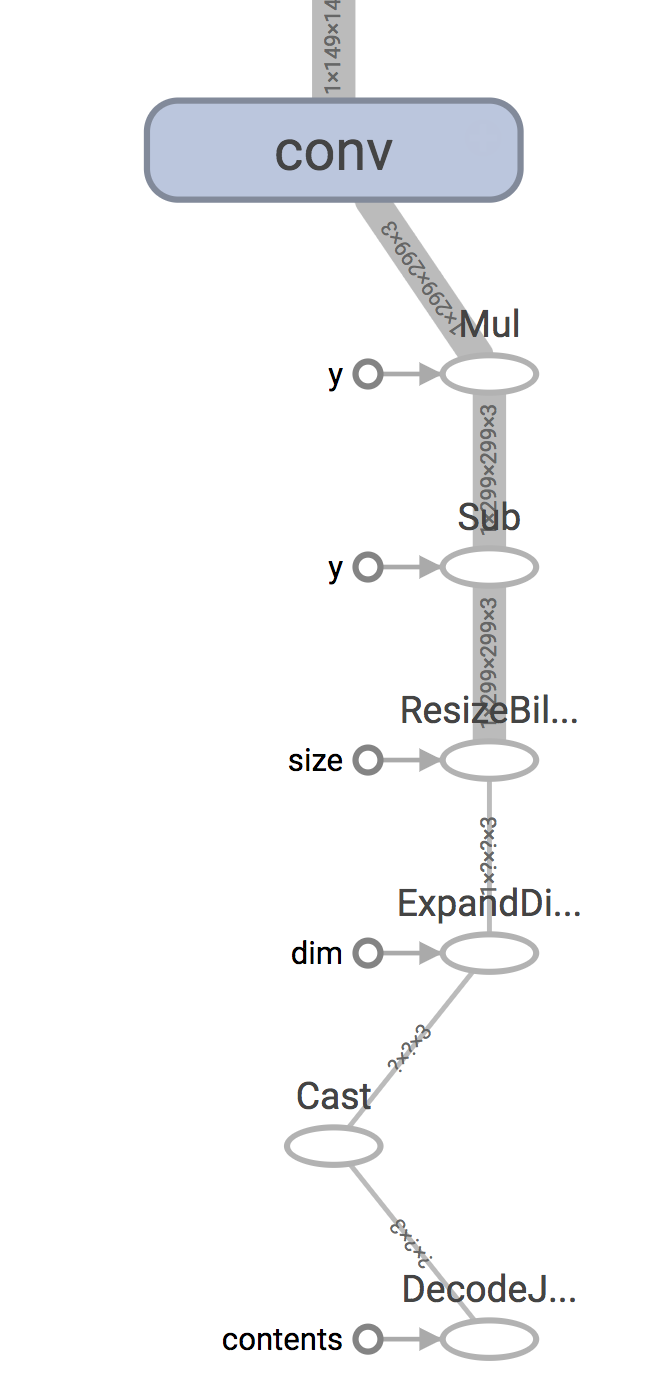
\includegraphics[scale=0.3]{inception_input.png}
\end{figure}
你需要做类似查看找出正确的输出节点。
如果你已经用一个frozen GraphDef文件,不确保内容尝试使用summarize\_graph工具打印出从图结构中找到的关于输入和输出的信息。这里是一个原始的Inception V3文件的例子
\lstinline[language=Bash]{bazel run tensorflow/tools/graph_transforms:summarize_graph -- i --in_graph=tensorflow_inception_graph.pb}
当你明白输入输出节点是什么,你可以分别对应--input\_names和--output\_names参数输入他们到图转化工具,调用strip\_unused\_nodes变换,如下:
\begin{lstlisting}
bazel run tensorflow/tools/graph_transforms:transform_graph --
--in_graph=tensorflow_inception_graph.pb
--out_graph=optimized_inception_graph.pb --inputs='Mul' --outputs='softmax'
--transforms='
  strip_unused_nodes(type=float, shape="1,299,299,3")
  fold_constants(ignore_errors=true)
  fold_batch_norms
  fold_old_batch_norms'

\end{lstlisting}
一件需要留心的是是你需要制定你想你的输入的大小和类型。这是因为一些你讲传入作为输入用于推理的值需要输入到特殊的Placeholder op操作,转如果他们不存在换也许需要创建他们,用Inception V3的例子,一个Placeholder节点取代以前的Mul节点用于输出resize和rescale图像矩阵。因此我们在调用TensorFlow之前正在处理我们自己。为了保留原始是的名字,这也是为什么我们总是在袖肥的Inception输入Mul然后运行一个session。
在你运行这个程序后,必将有一个仅仅包含需要运行预测程序的当前节点。在这点上在图上运行度量变得十分有用,因此他的值得再次运行summary\_graph明白在你的模型上有什么。
\subsection{什么操作应该被包含在移动端?}
在TensorFlow中有上百个可用的操作,每个操作针对不同的数据类型有多种实现。在移动平台编译后的二进制文件的大小非常重要,因为app捆绑下载的东西越小用户体验越好。如果所有的TensorFlow操作和数据类型被编译进入TensorFlow库中编译库可能有上10M,因此默认只有操作和数据类型的自己被包括。

这意味着如果你载入一个已经在桌面环境下训练过的模型文件,当你在移动平台载入它你也许看到No OpKernel was  registered to support Op错误。首先确保你删除了仅仅训练的节点,因为如果你的op从未执行错误将在载入时发生。如果当你照做后依然出现同样的问题,你将需要查看添加操作到你的构建库。

包含操作和类型的标准有如下类别:
\begin{itemize}
	\item 对于其他训练需要是否有用,比如checkpoint文件保存?我们丢弃它
	\item 是否以来的框架是移动端可用的,如libjpeg。避免额外的依赖,我们博包含DecodeJpeg操作
	\item 有不常使用的类型?我们不包含操作的boolean变量,因此我们不能在通常的推理图上看到他们中大多数
\end{itemize}
操作默认被修剪以适应移动平台的推理,但是可以修改构建文件修改默认。在修改构建文件后,你将需要重新编译TensorFlow。查看下面获取如何去做的更多细节,也可以查看\href{https://www.tensorflow.org/mobile/optimizing?hl=zh-cn#binary_size}{Optimizing}查看更多减小二进制文件尺寸的信息。
\subsection{定位实现}
操作被分为两部分。第一部分是操作的定义,什么操作的signature,那个输入,输出,拥有属性。这将占据非常小的空间,这些默认被包含。操作计算的实现在kernel(在tensorflor/core/kernels文件夹)中实现,你需要编译包含C++文件的内核实现进入库。为了找出那个文件是,你可以在源文件中搜索操作的名字。
\href{https://github.com/search?utf8=%E2%9C%93&q=repo%3Atensorflow%2Ftensorflow+extension%3Acc+path%3Atensorflow%2Fcore%2Fkernels+REGISTER+Mul&type=Code&ref=searchresults}{Here’s an example search in github}
你讲看到这个搜索正在寻找Mul操作实现,它在tensorflow/core/kernels/cwise\_op\_mul\_1.cc中。你需要用REGISTER开始寻找宏,你关心的操作的名字作为一个字符串参数。

在这种情况下,实现被才分为多个.cc文件,因此你需要在构建他们的过程中包含他们。如果你觉得用命令行搜索代码合适,这里是一个ghrep命令,如果你从TensorFlow仓库的跟目录运行它能定位正确的文件
\lstinline[language=Bash]{grep 'REGISTER.*"Mul"' tensorflow/core/kernels/*.cc}
\subsection{添加实现构建}
如果你用Bazel,为Android构建,你将需要添加文件\href{https://www.github.com/tensorflow/tensorflow/blob/r1.4/tensorflow/core/kernels/BUILD#L3565}{android\_extended\_ops\_group1}或者\href{https://www.github.com/tensorflow/tensorflow/blob/r1.4/tensorflow/core/kernels/BUILD#L3632}{android\_extended\_ops\_group2}目标。你也许需要包含任何的在这里依赖的.cc文件。如果构建报出缺少头文件,添加.h的文件到\href{https://www.github.com/tensorflow/tensorflow/blob/r1.4/tensorflow/core/kernels/BUILD#L3525}{android\_extended\_ops}。如果你用一个makefile在iOS,Raspberry Pi等等,去\href{https://www.github.com/tensorflow/tensorflow/blob/r1.4/tensorflow/contrib/makefile/tf_op_files.txt}{tensorflow/contrib/makefile/tf\_op\_files.txt}添加正确的实现文件。
\subsection{为移动端优化}
当你尝试部署在移动设备或者嵌入式设备上时,有一些特殊问题需要处理,当你部署你的模型的时候你将需要考虑他。

这些问题是:
\begin{itemize}
\item 模型和执行文件的大小
\item App速度和模型载入速度
\item 性能和线程
\end{itemize}
\subsection{TensorFlow 最低的设备要求是什么?}
你需要至少一兆的程序存储空间和多兆RAM运行基本的TensorFlow环境,因此对于DSP或者微控制器来说是不合适的。相比于这些,贵大的约束是设备的计算速度,和是否你能用较低的代价为你的应用运行模型。你可以在\href{https://www.tensorflow.org/mobile/optimizing?hl=zh-cn#how_to_profile_your_model}{How to Profile your Model}使用基准测试工具了解你的模型需要多少FLOPs,然后使用这个经验法则估计他们将在不同的设备上运行多快。例如,现代的智能手机也许有10GGLOPs/s,因此你希望从一个5GFLOP模型是每秒两帧,尽管你也许做的比较差的依赖同计算样板提取什么。

模型依赖是的在比较旧的或者资源少的手机上运行TensorFlow成为了可能。对更多的内存使用,我们通常需要确保TensorFlow创建的中间缓存不要太大,你也可以检查基准输出。

\subsection{Speed}
一个很高优先级的模型部署是找出五河更快的运行推理给出一个好的用户体验。首先是查看执行图要求的浮点操作。你可以使用benchmark\_model工具获取原始的估计。
\begin{lstlisting}[language=C++]
bazel build -c opt tensorflow/tools/benchmark:benchmark_model && \
bazel-bin/tensorflow/tools/benchmark/benchmark_model \
--graph=/tmp/inception_graph.pb --input_layer="Mul:0" \
--input_layer_shape="1,299,299,3" --input_layer_type="float" \
--output_layer="softmax:0" --show_run_order=false --show_time=false \
--show_memory=false --show_summary=true --show_flops=true --logtostderr
\end{lstlisting}
这将给你显示运行图需要多少操作。你也可以用这信息找出你的模型在目标上如何可行。例如,2016年出的高端手机能每秒到200亿FLOPs。因此你可能希望的罪加速度要求在大约500ms范围达到100亿 Flops。在想Rasphberry Pi3上可能有50亿Flops,你也许仅仅没两步得到一个推理。

有这些估计帮助你计划在设备上能湖区真是计算。如果迷行有太多操作,然后有一些机会优化架构减少数量。
高级的技术包含\href{https://arxiv.org/abs/1602.07360}{SqueezeNet} \href{https://arxiv.org/abs/1704.04861}{MobileNet}(针对移动设备快速但是牺牲少量精度)。你也可以查看一些可用的模型,及时老的模型,也许也很小。例如,Inception V1仅仅有700万参数,相比于Inception V3的240万参数,要求3亿FLOPs而不是v3的9亿参数。
\subsection{模型大小}
运行在设备上的模型需要被存储在设备上的某个地方,非常大的神经网络可能有数百兆。多数用户不愿从app store下载非常大的原件包,因此你想保证你的模型尽可能小。更进一步,越小的神经网络丝能在移动设备上运行的越快。
为了明白你磁盘上的网络多大,在上面(查看\href{https://www.tensorflow.org/mobile/prepare_models?hl=zh-cn}{Preparing models}了解更多关于这个工具的信息)运行freeze\_graph和strip\_unused\_nodes通过查看你的GraphDef的大小。因此当它仅仅包含推理相关的节点时。再次检查你的结果,运行summarize\_graph工具查看多少参数是常数:
\begin{lstlisting}[language=Bash]
bazel build tensorflow/tools/graph_transforms:summarize_graph && \
bazel-bin/tensorflow/tools/graph_transforms/summarize_graph \
--in_graph=/tmp/tensorflow_inception_graph.pb
\end{lstlisting}
这个命令应该给你类似下面的输出:
\begin{lstlisting}[language=Python]
No inputs spotted.
Found 1 possible outputs: (name=softmax, op=Softmax)
Found 23885411 (23.89M) const parameters, 0 (0) variable parameters,
and 99 control_edges
Op types used: 489 Const, 99 CheckNumerics, 99 Identity, 94
BatchNormWithGlobalNormalization, 94 Conv2D, 94 Relu, 11 Concat, 9 AvgPool,
5 MaxPool, 1 Sub, 1 Softmax, 1 ResizeBilinear, 1 Reshape, 1 Mul, 1 MatMul,
1 ExpandDims, 1 DecodeJpeg, 1 Cast, 1 BiasAdd 
\end{lstlisting}
我们当前意图的重要部分是常数参数的数量。在多数模型中讲被存储作为32位浮点数,因此如果你将参数乘上4,你应该得到接近磁盘上文件的大小。你可以用8位参数在最终的结果中损失很小的精度。因此如果你的文件太大你可以尝试使用\href{https://www.tensorflow.org/performance/quantization?hl=zh-cn}{quantize\_weights}减小参数:
\begin{lstlisting}[language=Bash]
bazel build tensorflow/tools/graph_transforms:transform_graph && \
bazel-bin/tensorflow/tools/graph_transforms/transform_graph \
--in_graph=/tmp/tensorflow_inception_optimized.pb \
--out_graph=/tmp/tensorflow_inception_quantized.pb \
--inputs='Mul:0' --outputs='softmax:0' --transforms='quantize_weights'
\end{lstlisting}
如果你查看结果文件的大小,你应该看到它有原来23M文件的1/4。

另一个变换是round\_weights,,它并不能是文件变得更小,但是它是文件能压缩quantize\_weights使用时的相同大小。他的特殊用途是移动部署,利用app在用户下载前安装包被压缩。

原始文件用标准的算法不能压缩的很好,因为一的数可能非常不同。round\_weights变换保持权重参数以浮点数存储,但是四舍五入他们到最近的值。这意味着存储的模型中有一些重复的字节模式,因此亚索可能带来尺寸的巨大减小,在一些情况下大小僵尸你作为8位存储。
round\_weights的另一个好处是框架不用分配临时buffer给解包的参数当我们必须的时候我们仅仅使用quantize\_weights。这保存一些时延(尽管结果应该被缓存以至于仅仅在第一次运行时花费)保证他能用内存映射,正如后面描述的。
\subsection{二进制文件的大小}
移动端和服务端最大不同是二进制文件的到校很重要。在桌面环境下它通常有上百兆,但是对于移动和嵌入式app保持二进制文件足够小以至于用户能轻松下载。正如上面提到的,TensorFlow包含默认操作实现的子集,但是最后的可执行文件仍然有12M。俄日了奸笑着,你可以建立你确实需要仅仅包含操作实现的库,基于自动分析你的模型。使用它。
\begin{itemize}
\item 在你的模型上运行tools/print\_required\_ops/print\_selective\_registration\_header.py生成使op能用的头文件
\item 放置ops\_to\_register.h文件到编译器能找到的路径。这可以是你的TensorFlow源文件的根目录。
\item 用SELECTIVE\_REGISTRATION定义构建TensorFlow,例如通过传递--copts="-DSELECTIVE\_REGISTERATION"到你的Bazel构建命令。
\end{itemize}
这个处理重新编译库以至于仅仅你需要的操作和类型被包含,这可能极大地减小可执行文件的大小。例如,结合Inception v3,新的大小仅仅1.5M。
\subsection{如何探测你的模型}
当你了解你的设备的峰值性能后,值得查看当前性能。使用表真的TensorFlow基准,而不是在更大的app中运行它,帮助隔离TensorFlow与时延。\href{https://www.github.com/tensorflow/tensorflow/blob/r1.4/tensorflow/tools/benchmark/}{tensorflow/tools/benchmark}工具设计用来帮助你做这个。为了在你的桌面机器中运行Inception V3,构架基准模型:
\begin{lstlisting}[language=Bash]
bazel build -c opt tensorflow/tools/benchmark:benchmark_model && \
bazel-bin/tensorflow/tools/benchmark/benchmark_model \
--graph=/tmp/tensorflow_inception_graph.pb --input_layer="Mul" \
--input_layer_shape="1,299,299,3" --input_layer_type="float" \
--output_layer="softmax:0" --show_run_order=false --show_time=false \
--show_memory=false --show_summary=true --show_flops=true --logtostderr 
\end{lstlisting}
你应该看到类似下面的输出:
\begin{lstlisting}[language=Bash]
============================== Top by Computation Time ==============================
[node
 type]  [start]  [first] [avg ms]     [%]  [cdf%]  [mem KB]  [Name]
Conv2D   22.859   14.212   13.700  4.972%  4.972%  3871.488  conv_4/Conv2D
Conv2D    8.116    8.964   11.315  4.106%  9.078%  5531.904  conv_2/Conv2D
Conv2D   62.066   16.504    7.274  2.640% 11.717%   443.904  mixed_3/conv/Conv2D
Conv2D    2.530    6.226    4.939  1.792% 13.510%  2765.952  conv_1/Conv2D
Conv2D   55.585    4.605    4.665  1.693% 15.203%   313.600  mixed_2/tower/conv_1/Conv2D
Conv2D  127.114    5.469    4.630  1.680% 16.883%    81.920  mixed_10/conv/Conv2D
Conv2D   47.391    6.994    4.588  1.665% 18.548%   313.600  mixed_1/tower/conv_1/Conv2D
Conv2D   39.463    7.878    4.336  1.574% 20.122%   313.600  mixed/tower/conv_1/Conv2D
Conv2D  127.113    4.192    3.894  1.413% 21.535%   114.688  mixed_10/tower_1/conv/Conv2D
Conv2D   70.188    5.205    3.626  1.316% 22.850%   221.952  mixed_4/conv/Conv2D

============================== Summary by node type ==============================
[Node type]  [count]  [avg ms]    [avg %]    [cdf %]  [mem KB]
Conv2D            94   244.899    88.952%    88.952% 35869.953
BiasAdd           95     9.664     3.510%    92.462% 35873.984
AvgPool            9     7.990     2.902%    95.364%  7493.504
Relu              94     5.727     2.080%    97.444% 35869.953
MaxPool            5     3.485     1.266%    98.710%  3358.848
Const            192     1.727     0.627%    99.337%     0.000
Concat            11     1.081     0.393%    99.730%  9892.096
MatMul             1     0.665     0.242%    99.971%     4.032
Softmax            1     0.040     0.015%    99.986%     4.032
<>                 1     0.032     0.012%    99.997%     0.000
Reshape            1     0.007     0.003%   100.000%     0.000

Timings (microseconds): count=50 first=330849 curr=274803 min=232354 max=415352 avg=275563 std=44193
Memory (bytes): count=50 curr=128366400(all same)
514 nodes defined 504 nodes observed
\end{lstlisting}
这是总结的视图,他能通过show\_summary标记显示。为了解释他首先表格是一个节点花费时间的列表。花费时间的排序,从左到右,列是:
\begin{itemize}
\item 节点类型,操作的种类
\item op的开始时间,显示序列操作在哪里下降
\item 首先是毫秒,是第一次运行基准测试花费了多少时间,因此通过博人20运行是执行得到可行的统计。第一次对于发现操作计算花费很有用,然后缓存数据
\item 所有运行的操作的平均时间,毫秒
\item 运行op占据的总时间的百分比。对于理解热点在哪里很有用。
\item 之前所有表格中操作的时间。他对于理解层中什么分布式的工作,查看多少节点花费了大多数的时间很有用
\item 节点的名字
\end{itemize}
第二个表格类似但是通过类似节点才分时间,通过op的种类组合他们。这对于理解那个操作实现想要优化或者从表中消除是很有用的。表格从开始排列多数费时的操作,仅仅显示前10个入口,对于其他的节点结合placeholder,列从左往右是:
\begin{itemize}
\item 典型被分析的节点
\item 这种类型所有节点的累计平均时间,毫秒
\item 操作类型总共时间的多少比例被花费
\item 比这个操作类型更高的累计时间花费,因此你可以理解workload的分布
\item 这个输出的多少内存被占用
\end{itemize}
两个建立的表格使得你能很容易的复制和粘贴他们的结果到电子表格文件,因此他们被介个tabs作为列的分割输出。通过节点类型的总结当查找油画机会可能很有用,因为它是代码花费时间的关键点。在这种情况下,你可能看到Conv2D操作大约90\%的执行时间。这是一个图优化的符号,因为卷积和举着成是神经网络的计算workload。
正如经验指出,更多的考虑如果你查看一些其他的操作占据超过一个晓得时间比例。对于神经网络,通常不涉及大矩阵乘法通常应该比单个小,因此如果你的一些时间进入了这里,这意味着你的网络不是一个有花的结构,或者实现这些操作的代码没有优化到它能优化的底部。如果你看到这些情况总是欢迎你查看\href{https://github.com/tensorflow/tensorflow/issues}{Performance bugs }或者patch,特别是如果你包含一个附件模型展示这个行为和命令行用于在基准测试工具上运行。

为了在左面环境上运行下面,但是这个工具在Android上工作,这对于移动部署很有用,下面的在arm64bit上运行示例的命令:
\begin{lstlisting}[language=Bash]
bazel build -c opt --config=android_arm64 \ 
tensorflow/tools/benchmark:benchmark_model
adb push bazel-bin/tensorflow/tools/benchmark/benchmark_model /data/local/tmp
adb push /tmp/tensorflow_inception_graph.pb /data/local/tmp/
adb shell '/data/local/tmp/benchmark_model \
--graph=/data/local/tmp/tensorflow_inception_graph.pb --input_layer="Mul" \
--input_layer_shape="1,299,299,3" --input_layer_type="float" \
--output_layer="softmax:0" --show_run_order=false --show_time=false \
--show_memory=false --show_summary=true'
\end{lstlisting}
你可以用和桌面满相同的方法解释上面的命令,如果你对于找出输入输出名字和类型有点麻烦查看\href{https://www.tensorflow.org/mobile/prepare_models?hl=zh-cn}{Preparing models}页默认关于你的模型如何检测这些,查看summarize\_graph工具也许给你一些帮助信息。

这不支持iOS下的命令行,因此在\href{https://www.github.com/tensorflow/tensorflow/blob/r1.4/tensorflow/examples/ios/benchmark}{tensorflow/examples/ios/benchmark}中有一个分割的例子,包的功能和标准app的功能相同。食醋胡统计设备屏幕和调试日志。如果你想为Android例子在屏幕上统计,你可以通过按压音量上键打开他们。

\subsection{探测你的app}
你通过benchmark工具查看的从模型生成的输出包含作为标准TensorFlow的一部分,这意味着你必须在你自己的应用中访问他们,你可以查看一个\href{https://www.github.com/tensorflow/tensorflow/blob/r1.4/tensorflow/examples/ios/benchmark/BenchmarkViewController.mm?l=139}{例子}

基本的步骤是:
\begin{itemize}
\item 创建StatSummarizer对象\lstinline[language=C++]{tensorflow::StatSummarizer stat_summarizer(tensorflow_graph);}
\item 建立选项:
\begin{lstlisting}[language=Python]
tensorflow::RunOptions run_options;
run_options.set_trace_level(tensorflow::RunOptions::FULL_TRACE);
tensorflow::RunMetadata run_metadata;
\end{lstlisting}
\item 运行图:
\begin{lstlisting}[language=Python]
run_status = session->Run(run_options, inputs, output_layer_names, {},
                          output_layers, &run_metadata);

\end{lstlisting}
\item 计算打印结果\begin{lstlisting}[language=Python]
assert(run_metadata.has_step_stats());
const tensorflow::StepStats& step_stats = run_metadata.step_stats();
stat_summarizer->ProcessStepStats(step_stats);
stat_summarizer->PrintStepStats();
\end{lstlisting}
\end{itemize}
\subsection{可视化模型}
多数搞笑的加速你的代码的方法是通过修改你的模型因为它做很少的工作。左到这个你需要明白你的模型在做什么,可视化它是一个好的一步。为了获取高级图概览,使用\href{https://github.com/tensorflow/tensorboard}{TensorBoard}
\subsection{线程}
TensorFlow桌面环境有一个高级的县城模式,如果可以将尝试运行多个操作。在我们的在我们的属于李成为"Inter-op parallelism"(烤炉避免和"intra-op"弄混,你可以把他当做"between-op"),你可以通过在会话选项中指定inter\_op\_parallelism\_threads。

默认,移动设备连续的运行操作,这是inter\_op\_parallielism\_threads被设置为1。移动处理器通常有一些核心很小的的cache,因此运行多个互不影响在分开的内存区域对性能没有帮助。"Intra-op parallelism"或者("Within-op")可能很有用,特别是对于计算受限的操作想卷积(不同的线程可以输入相同的小的存储区)。

在移动端,一个操作多少线程将被使用同默认设置核心数,或者当核心不被决定的时候为2。你可以在会话选项设置intra\_op\_parallelism\_threads覆盖默认的线程数。如果你有自己的线程处理繁重的任务一个好的想法是减少默认线程数量,一直以他们不能相互影响。为了查看更多会话选项,查看\href{https://www.github.com/tensorflow/tensorflow/blob/r1.4/tensorflow/core/protobuf/config.proto}{ ConfigProto}
\subsection{使用移动数据重新训练}
在移动app上运行模型的一个最大的问题是精度不能代表训练数据。例如,多数ImageNet照片well-gramed以至于对象在图片的中铁建,well-lit和正规lens的shot。手机设备上的相片经常帧率低,badly lit,可能有鱼眼畸变。

解决方案是扩展从你的应用捕获的训练集。这步设计额外的工作,因此你将必须自己标记样本,但是及时你用它扩展你的原始的训练数据,他可能对训练数据集有帮助。为了通过做这个改善训练集合,通过福鼎其他的想复制或者差的标签样本修复其他的质量问题是最好的提升精度分方法。通常比使用不同的技术修改你的模型架构更有效。
\subsection{减少模型载入时间和内存footprint}
大多数的操所系统运与你用内存映射载入一个文件,而不是通过通常的I/O API。相对于在堆上分配一个内存区域而是从磁盘复制字节进去,你简单的高数操作系统使得文件的整个内容在内存中出现。这有一些好处:
\begin{itemize}
\item 载入速度
\item 减少page(增加性能)
\item 不为你的app计数RAM预算
\end{itemize}
TensorFlow也支持能从一些模型文件映射权重。因为在ProtoBuf序列化格式的限制,我们必须改变我们的模型载入和处理代码。这个内存映射工作是我们有一个文件,第一部分是正常GraphDef序列为protocol buffer wire格式,但是权重以一种方式添加以至于能被直接映射。
为了创建这个文件,运行tensorflow/contrib/util:conver\_graphdef\_memmapped\_format工具。这接受在GraphDef文件通过freeze\_graph运行,转化它到权重被添加到最后的格式。因此文件不在是一个标准的GraphDef protobuf,你需要做一些改变载入代码。你可以在LoadMemoryMappedModel()函数中\href{https://www.github.com/tensorflow/tensorflow/blob/r1.4/tensorflow/examples/ios/camera/tensorflow_utils.mm?l=147}{iOS Cammera demo app}查看这个例子。

同样的代码(结合Object C调用获取文件的过去文件的替代)可以用在其他的平台。因为我们用内存银蛇,我们需要通过创建一个特殊的TensorFlow环境对象监理文件我们将使用:
\begin{lstlisting}[language=C++]
std::unique_ptr<tensorflow::MemmappedEnv> memmapped_env;
memmapped_env->reset(
      new tensorflow::MemmappedEnv(tensorflow::Env::Default()));
tensorflow::Status mmap_status =
      (memmapped_env->get())->InitializeFromFile(file_path);
\end{lstlisting}
你然后需要在这个环境传递子序列,唱着歌载入图:
\begin{lstlisting}[language=C++]
tensorflow::GraphDef tensorflow_graph;
tensorflow::Status load_graph_status = ReadBinaryProto(
    memmapped_env->get(),
    tensorflow::MemmappedFileSystem::kMemmappedPackageDefaultGraphDef,
    &tensorflow_graph);
\end{lstlisting}
你也需要创建会话结合一个指针到环境:
\begin{lstlisting}[language=C++]
tensorflow::SessionOptions options;
options.config.mutable_graph_options()
    ->mutable_optimizer_options()
    ->set_opt_level(::tensorflow::OptimizerOptions::L0);
options.env = memmapped_env->get();

tensorflow::Session* session_pointer = nullptr;
tensorflow::Status session_status =
    tensorflow::NewSession(options, &session_pointer);

\end{lstlisting}
这里有一件事需要注意,我们禁用了自动优化,因此在一些情况下,浙江折叠子树,创建一个tensor值的复制(我们不想用更多的RAM)

当你进行这些步的时候,你可以用session和graph作为normal,你应该看到载入时间和内存使用减小。

\subsection{从简单的复制保护模型文件}
默认,你的模型将从一个被存在磁盘上标准的序列化的protobuf。理论上任何人可以复制你的模型,你也许不想这样。然而,实际上多数模型通过优化变得如此专用和混淆,风险类似在竞争者反编译和重瞳你的代码,但是如果你想使得他结合普通的用户访问你的文件是不可能的采用如下步骤。

我们多数代码使用\href{https://www.github.com/tensorflow/tensorflow/blob/r1.4/tensorflow/core/platform/env.cc?q=core/platform/env.cc&l=409}{ReadBinaryProto()}方便的调用从磁盘载入GraphDef。这要求一个没有加密的protobuf。幸运的,调用实现是相当直接应该很容易在内存中写一个等价可以加密的。这里一些代码显示你可以使用自己的加密环境如何读和加密一个protobuf。
\begin{lstlisting}[language=C++]
Status ReadEncryptedProto(Env* env, const string& fname,
                          ::tensorflow::protobuf::MessageLite* proto) {
  string data;
  TF_RETURN_IF_ERROR(ReadFileToString(env, fname, &data));

  DecryptData(&data);  // Your own function here.

  if (!proto->ParseFromString(&data)) {
    TF_RETURN_IF_ERROR(stream->status());
    return errors::DataLoss("Can't parse ", fname, " as binary proto");
  }
  return Status::OK();
}
\end{lstlisting}
为了使用这,你将需要定义一个DecryptData()函数。他可能想下面这样简单:
\begin{lstlisting}[language=C++]
void DecryptData(string* data) {
  for (int i = 0; i < data.size(); ++i) {
    data[i] = data[i] ^ 0x23;
  }
}

\end{lstlisting}
你也许想要一些更复杂的,但是明确你将需要当前scope外的什么?





































 
\section{对于ML初学者的MNIST}
这个导航针对于对机器学习和TensorFlow生疏的读者。如果你知道MNIST,softmax回归,你最好查看\href{https://www.tensorflow.org/get_started/mnist/pros}{faster paced turotial}。开始任何导航前确保你安装了\href{https://www.tensorflow.org/install/index}{TensorFlow}。
当一个人学习如何编程,他们通常做的第一件事就是打印Hello World。MNIST对于机器学习就像编程的Hello World。

MNIST是一个简单的计算机视觉数据集,由像下面的手写数据组成:
\begin{figure}[H]
\centering

\includegraphics{MNIST.png}
\caption{mnist数据}
\end{figure}
它包含每个图片的标签,高数我们是那个数字。例如,上面的标签分别是5,0,4,1。

在这个导航中,我们将训练一个模型查看图像预测数字。我们的目标不是训练一个真正精巧的模型获取顶尖的性能,尽管我们将在稍后给你代码。但是不是使用TensorFlow简单研究。例如,我们将开始一个非常简单的称为Softmax回归的模型。

实际上代码很短,所有有趣的东西仅仅发生在三行。然而,对于理解它背后的想法却很重要:TensorFlow如何工作和机器学习核心概念。因为这,我们将分厂自己的介绍代码。
\subsection{关于这个导航}
这个导航是一个一行行的解释\href{https://www.github.com/tensorflow/tensorflow/blob/r1.4/tensorflow/examples/tutorials/mnist/mnist_softmax.py}{mnist\_softmax.py}发生了什么。你可以通过两种不同的方法使用这个导航:
\begin{itemize}
\item 当你读每一行解释的时候复制粘贴一行行的每个代码段到Python环境
\item 在你读整个解释致歉运行整个mnist\_softmax.py Python文件,使用导航理解你不清楚的每行代码
在这个导航你将完成:
\item 了解MNIST数据集和softmax回归
\item 创建一个函数模型用于识别,易于图片上的每个像素
\item 通过"看"样本使用TensorFlow训练模型识别数字(运行我们的TensorFlow会话做到)
\item 结合我们的测试数据检查模型的精度
\end{itemize}
\subsection{MNIST数据}
MNIST数据在\href{http://yann.lecun.com/exdb/mnist/}{Yann LeCun's website}。如果你从文档上复制粘贴代码,用下面两行代码开头自动下载读取数据:
\begin{pythoncode}
from tensorflow.examples.tutorials.mnist import input_data
mnist = input_data.read_data_sets("MNIST_data/", one_hot=True)
\end{pythoncode}
MNIST数据分为3部分:55,000训练数据(mnist.train),10,000测试数据(mnist.test)和5,000验证数据(mnist.validation)。这分割很重要:它是机器学习中的基础用来分割数据以至于在没有学习的数据上学到实际上的范化。

正如 我们之前提到的,每个MNIST数据有两部分:手写数字的图片和对应的标签。我们将称为图像"x"和标签"y"。训练集和测试机都包含图像和对应的标签;例如训练图像是mnist.train.images训练标签是mnist.train.labels。

每张图片有$28\times28$像素,我们可以将他解释为一个数组:
\begin{figure}[H]
\centering
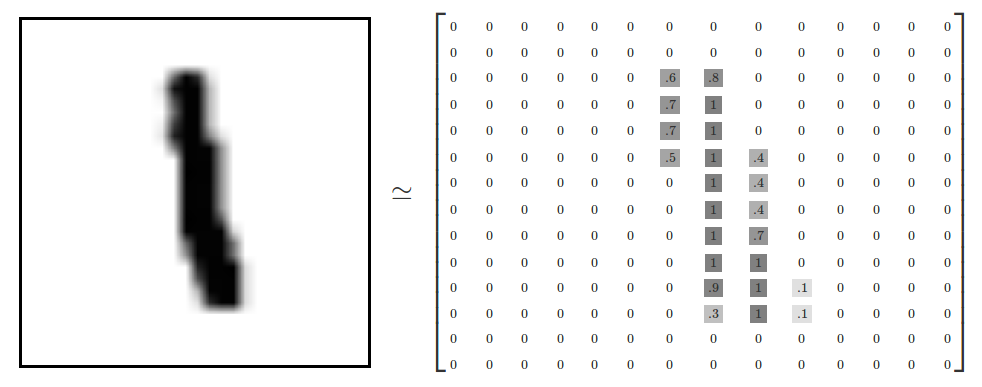
\includegraphics[scale=0.2]{MNIST-Matrix.png}
\caption{图片和对应的矩阵}
\end{figure}
我们可以展开这个数组为一个$28\times28=784$个数的向量。我们如何展开数组不重要只要它和图像一致即可。从这个观点,MNIST图像仅仅是一个\href{https://colah.github.io/posts/2014-10-Visualizing-MNIST/}{very rich structure }784维的向量空间。(警告:计算加强可视化)

展开市局丢掉了图像的2D结构,这很不好?使得最佳的计算机视觉方法利用这个结构,我们将在后面的导航中看到。但是简单的方法softmax回归将在这里使用。

结果时mnist.train.images是一个形状为[55000,784]的tensor(n维)。第一个为都市图像的索引,第二个是索引对应的图像像素。图像中的像素每个tensor的输入是一个0或者1。
\begin{figure}[H]
\centering

\includegraphics[scale=0.2]{mnist-train-xs.png}
\caption{图像维度}
\end{figure}
每个MNIST中的图像有一个对应的标签,一个0-9的数字,为了达到导航的目的,我们转化我们的标签为“one-hot vector”。一个one-hot向量是一个多数维度上为0,一个维度上1的向量。这种情况下,第n个数字表示维度中第n位置为1.例如3应该是[0,0,0,1,0,0,0,0,0,0]。结果mnist.train.labels是一个[55000,10]的浮点数组。
\begin{figure}[H]
\centering

\includegraphics[scale=0.2]{mnist-train-ys.png}
\caption{one-hot vector}
\end{figure}
现在我们准备开始我们的模型。
\subsection{Softmax回归}
我们知道在MNIST中的每张图片是0-9的手写体。因此给定一张图片仅仅只有10个可能。我们想能查看一张图片给定每张图片的概率。例如,我们的模型也许查看图像9 80\%确定是9,5\%确定为8其他的可能性很小因为模型不能100\%确定。

对这个经典的问题softmax恢复是一个自然,简单的模型。如果你想复制概率给一个对象成为多个不同对象中的一个,softmax做的就是这个,因为softmax给0-1的输出。在之后当我们训练更加精妙的模型,最后的步骤将是一个softmax操作。

一个softmax回归有两部:首先我们添加在确定类别中的输入,然后我们转化输出概率。为了总结一个类别的概率,如果它被支持我们权衡像素强度。

下面的图显示了从这些类别权衡一个模型。红色表示负权重,蓝色表示正权重。

\begin{figure}[H]
\centering
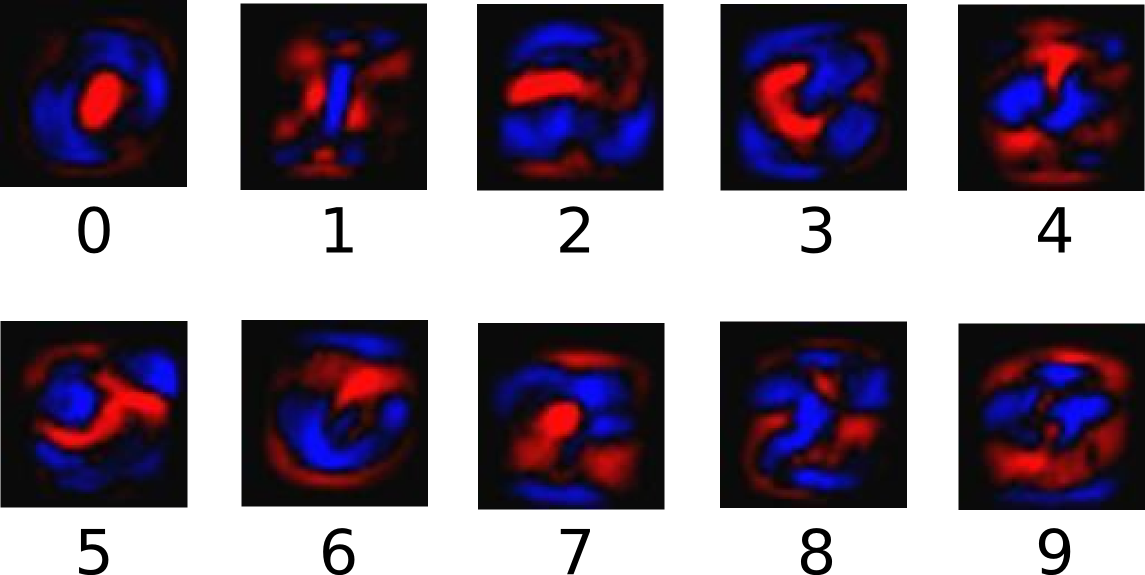
\includegraphics[scale=0.2]{softmax-weights.png}
\caption{softmax手写体}
\end{figure}
我们添加额外的偏执。基本上,我们想能说一些事更可能和输入独立。结果时给定输入x了类别i结果是:
\[evidence_i = \sum_{j}W_{i,j}x_j+b_i\]
这里的$W_i$是权重$b_i$是类别i偏置,j是在我们的输入图像x上的求和的索引。我们使用softmax转化evidence为我们的预测概率y:
\[y=softmax(evidence)\]
这里的softmax作为一个激活函数或者链接函数,输出我们线性函数为我们想要的。在这种情况下,概率分布在10个类别上。我们可以认为转化依据为我们输入每个类别的概率,定义如下:
\[softmax(evidence)=normalize(exp(evidence))\]
如果你展开方程,你得到:
\[softmax(evidence)_i = \frac{exp(evidence_i)}{\sum_jexp(evidence_j)}\]
但是首先考虑softmax方法京城很有用:指数输入和归一化。指数平均一个单元增加权重到任何假设。相反有更少的证据意味着假设获取之前前中的一部分。没哟偶假设有0或者负权重。fostmax然后归一化权重,以至于相加为1。形成一个可用的概率分布。(为了说明softmax函数,查看Michael Nielsen的数的\href{http://neuralnetworksanddeeplearning.com/chap3.html#softmax}{章节},完全的交互式可视化。)

你可以想下面画softmax回归,尽管有更多的x。对于每个输入,我们计算x的加权和加上偏执使用softmax。
\begin{figure}[H]
\centering
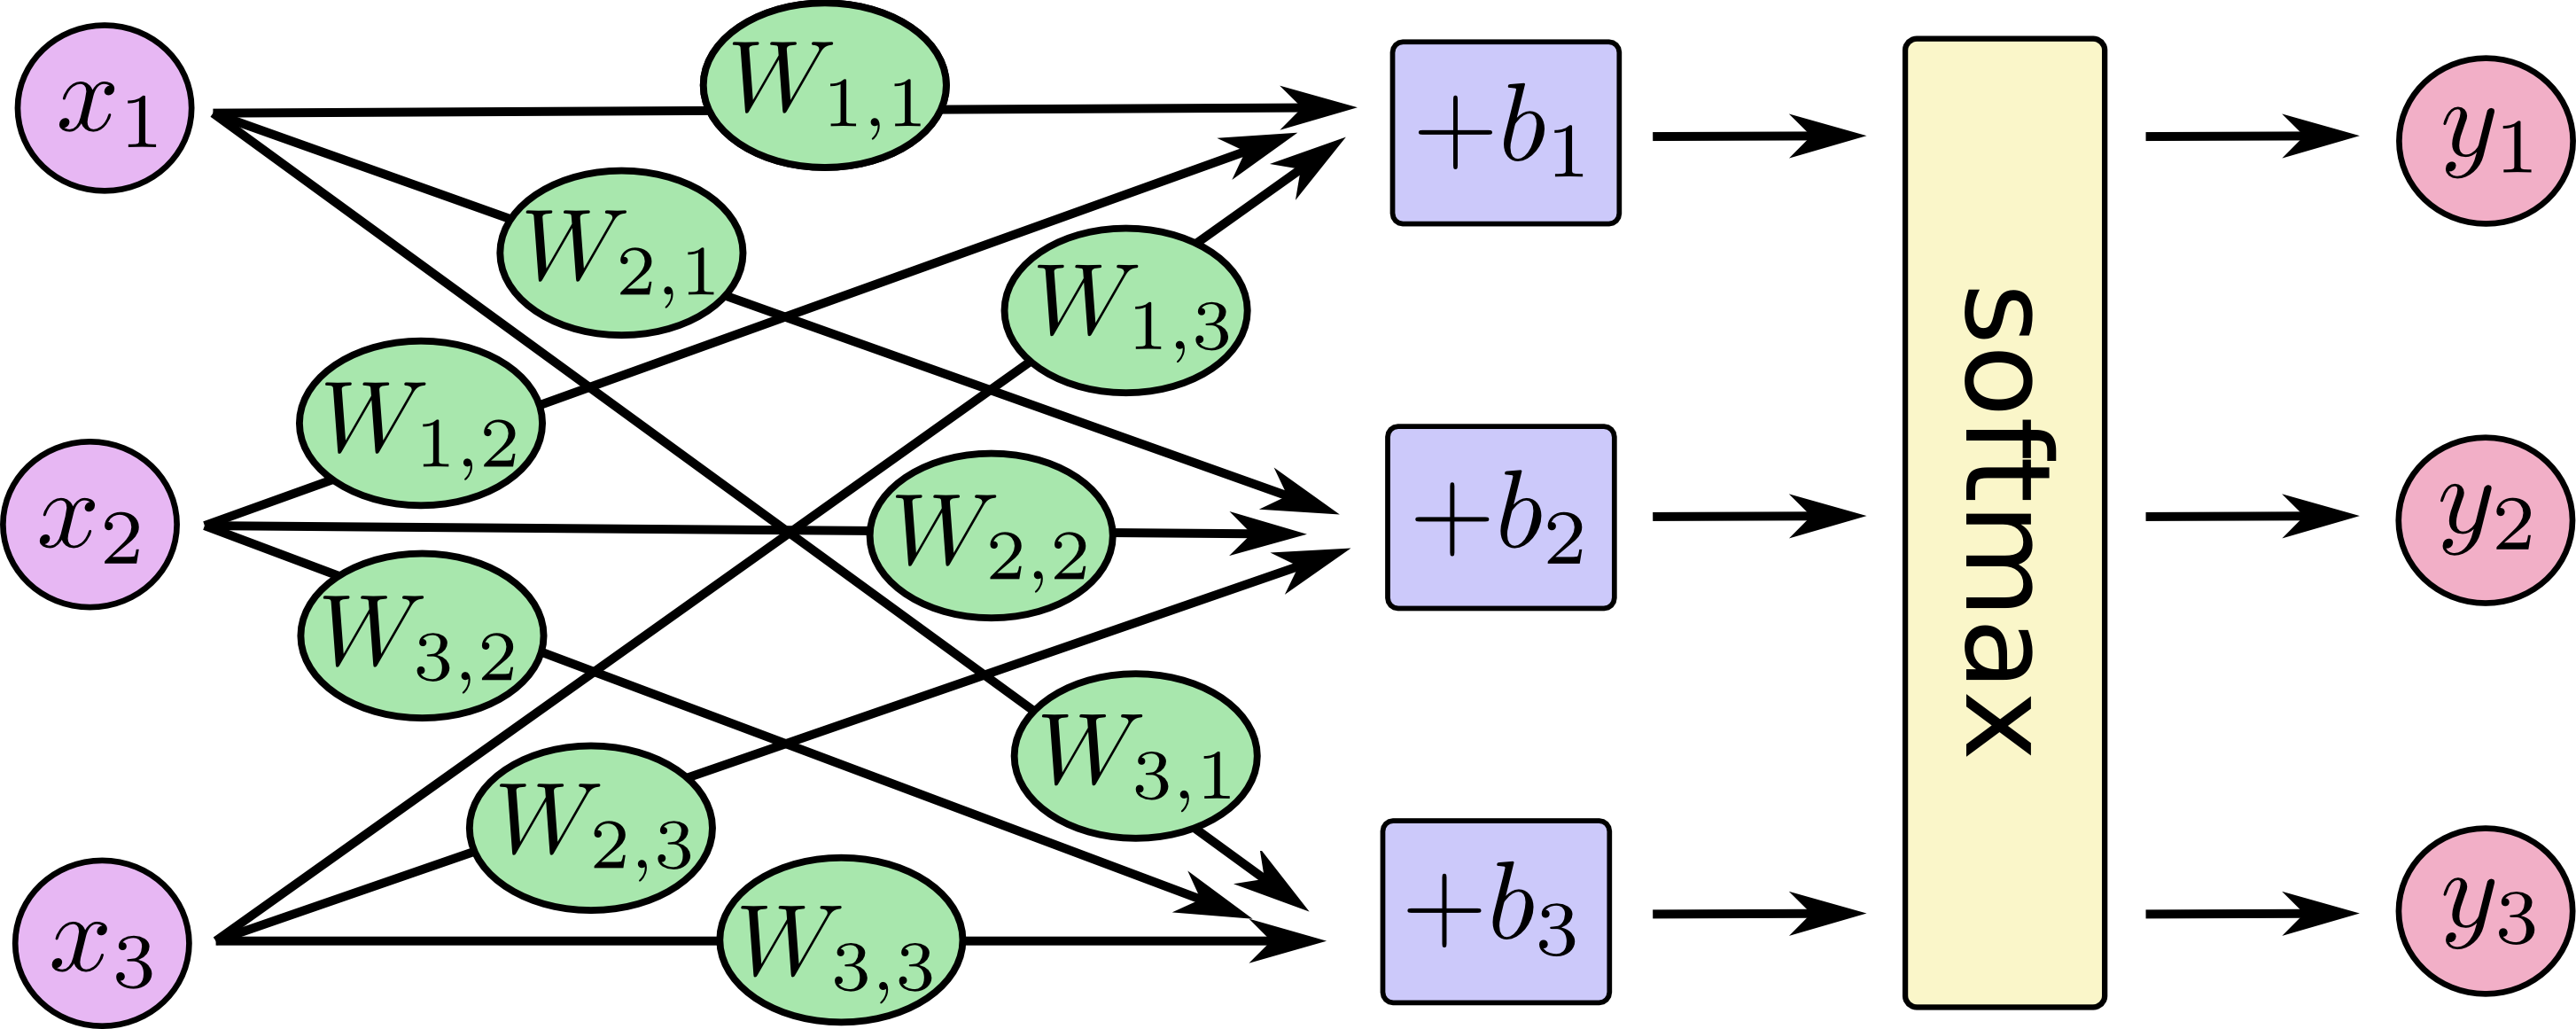
\includegraphics[scale=0.1]{softmax-regression-scalargraph.png}
\caption{softmax计算过程}
\end{figure}
如果你写为方程,你得到:
\begin{figure}[H]
\centering
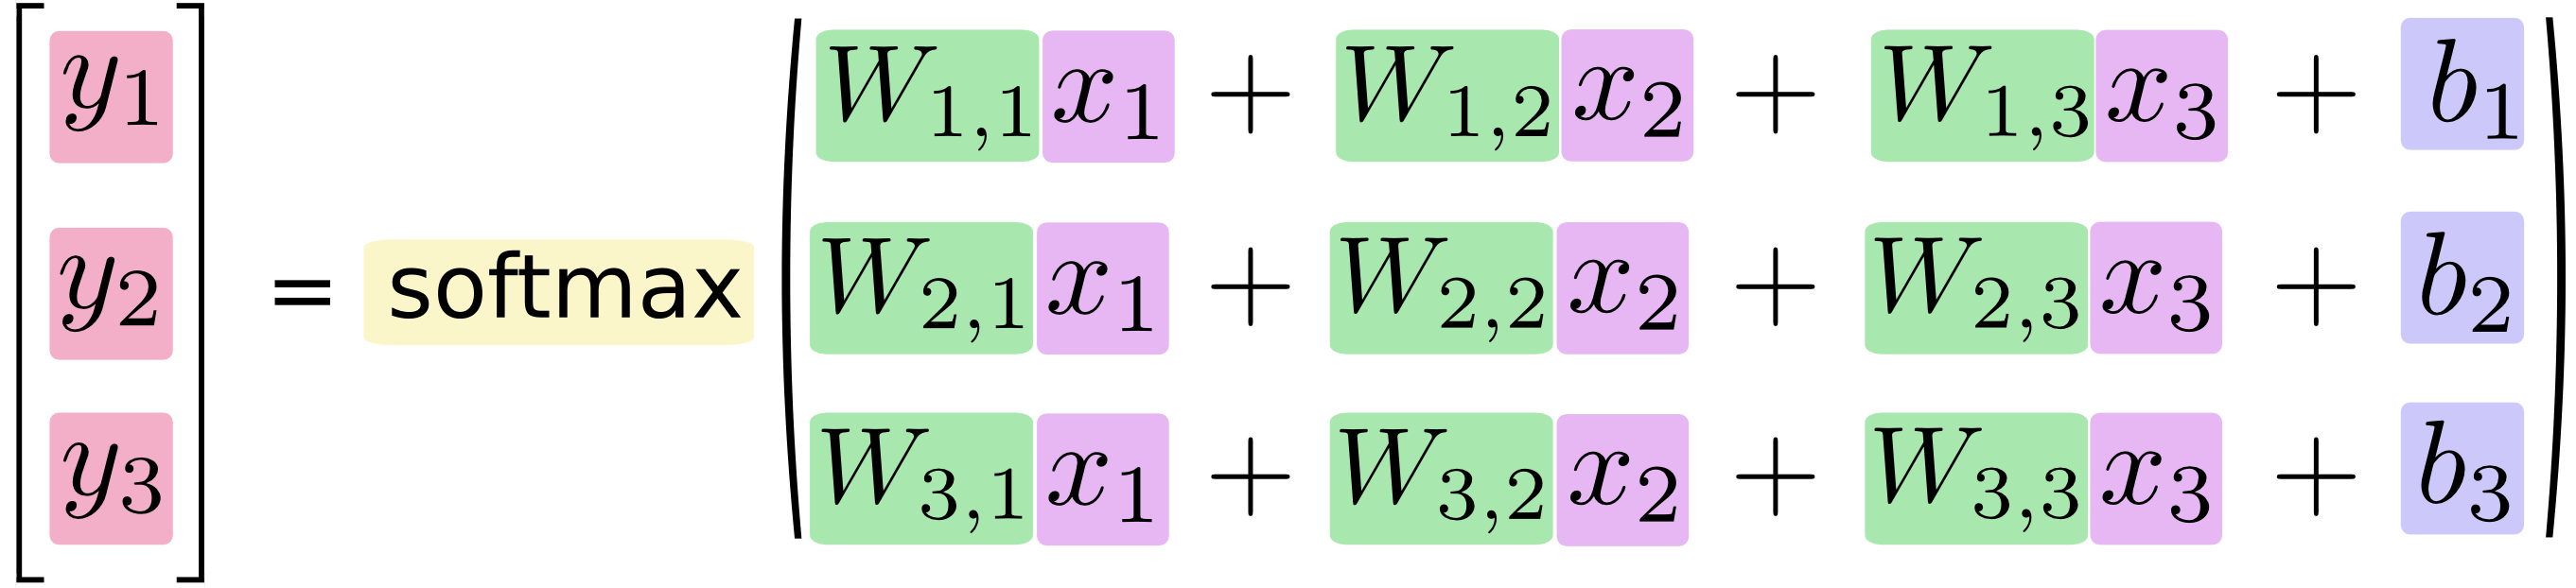
\includegraphics[scale=0.1]{softmax-regression-scalarequation.png}
\caption{softmax 方程}
\end{figure}
我们可以向量化这个过程,转变他为一个矩阵惩罚和向量加。这对于高效计算很有用(它总是一个有用的思考方法)。
\begin{figure}[H]
\centering
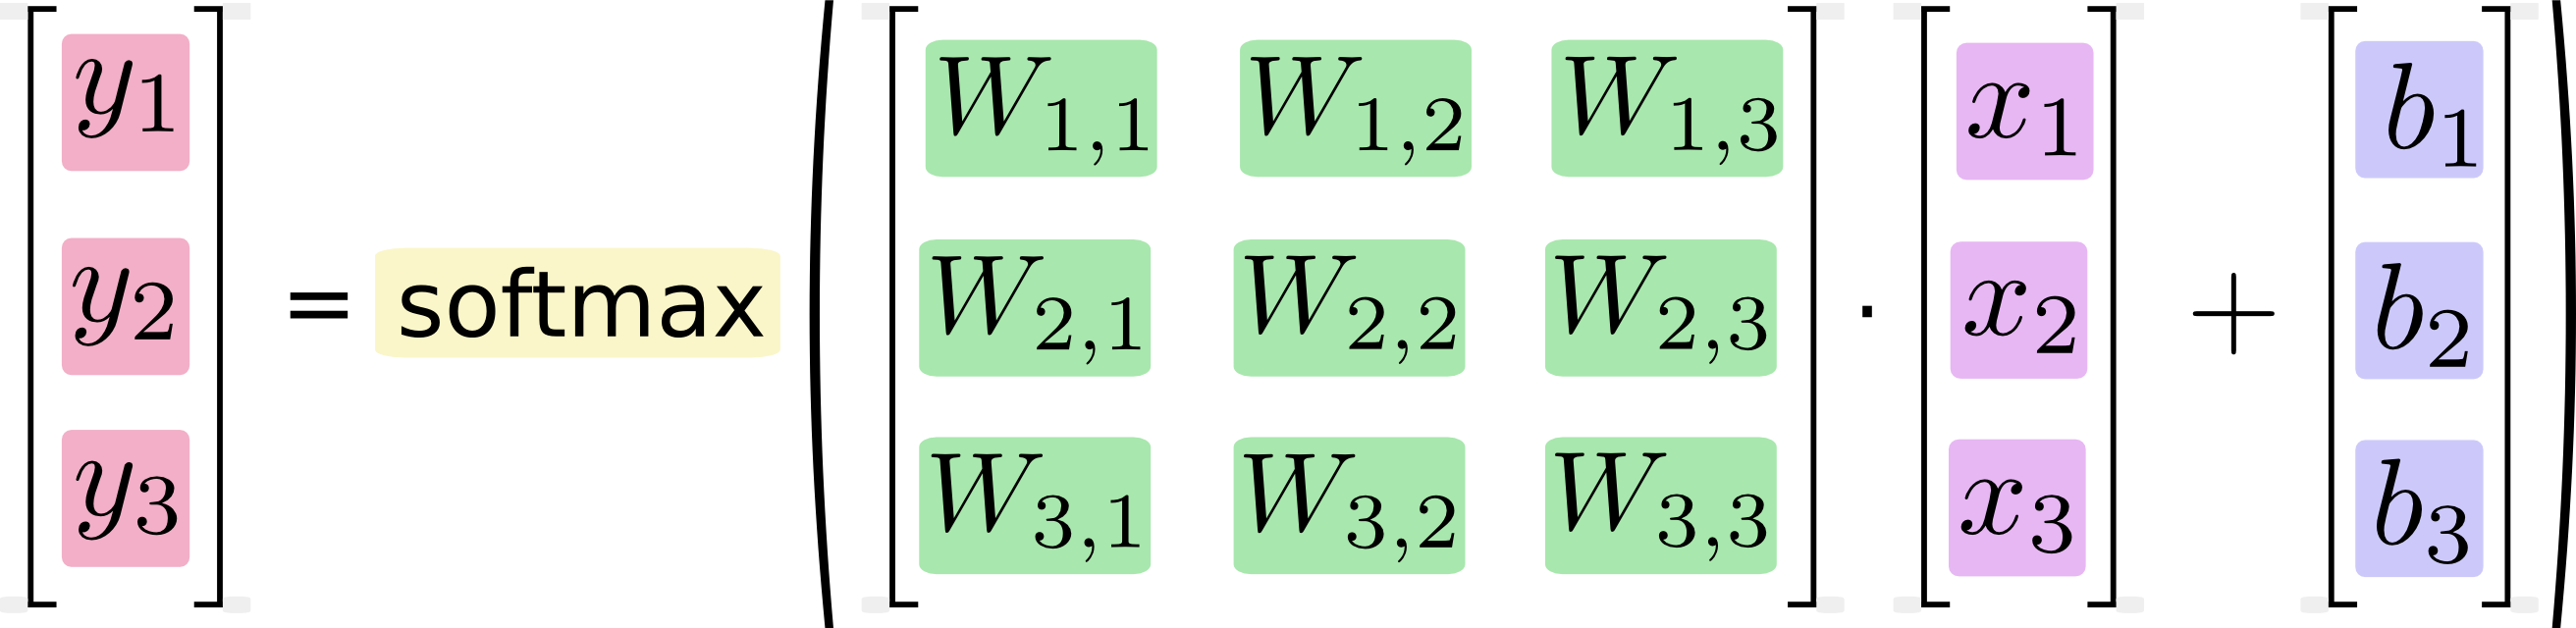
\includegraphics[scale=0.1]{softmax-regression-vectorequation.png}
\caption{向量化的softmax}
\end{figure}
更加简洁的你可以这样写:
\[y=fostmax(Wx+b)\]
现在我们使用TensorFlow转化它。
\subsection{实现回归}
为了在Python中进行的数值计算,我们通常使用一个\href{http://www.numpy.org/}{NumPy}库在Python外使用其他其他语言的高效实现做代价高昂的矩阵乘法操作。不幸的是转化每个操作会Python的时候依然有一些开销。如果你在GPU或者是分布式环境(这里我们转化数据代价很高)中使用是开销特别大。

TensorFlow也在Python外做了提升,但是对于减小开销减少有一点作用。想不语从Python运行的代价,TensorFlow让我们在Python外描述交互的操作。(这样的方法可以在一些机器学习库中看到)

为了使用TensorFlow,首先导入他。
\begin{ipythoncode}
import tensorflow as tf 
\end{ipythoncode}
我们通过符号变量描述交互的操作,让我们创建一个:
\begin{ipythoncode}
x = tf.placeholder(tf.float32, [None, 784])
\end{ipythoncode}
x没有指定值。是一个当我们要求TensorFlow运行时放置值的placholder。我们想能输入任意数量的MNIST图像,每张图像展开为784维(这里的None意味着这一维度可以为任意长度)
我们也需要权重和偏执用于计算。我们可以想象这些为额外的输入,但是TensorFlow有更好的处理方法:Variable。一个Variable是在TensorFlow图上的交互操作的一个可修改的tensor。他可以通过计算使用和修改。对于机器学习应用,一个常规的模型参数为Variable。
\begin{pythoncode}
W = tf.Variable(tf.zeros([784, 10]))
b = tf.Variable(tf.zeros([10]))
\end{pythoncode}
我们通过tf.Variable创建这些Variable初始化variable的值:在这种情况下,我们初始化W和b作为全0 tensor。因此我们将学习W和b。他们初始化为什么不重要。注意W形状为[784,10]因为我们想乘784维图像向量生成10维不同类别可信向量。b形状为[10]因此可以添加到输出。我们可以用一行定义实现我们的模型:
\begin{pythoncode}
y = tf.nn.softmax(tf.matmul(x, W) + b)
\end{pythoncode}
首先我们用tf.matmul(x,w)乘上x和W。它可我们方程用颠倒了这里是$Wx$作为结合多输入一个处理x为2D tensor的技巧。我们然后添加b最后使用tf.nn.softmax

这里我们使用了一行定义我们的模型,之后的一些行设置。这是不是因为TensorFlow设计就是为了做一个特别容易的regression:它仅仅是一个灵活的描述一些种类数值计算的方法,通过机器学习模型护理方针。一旦定义,我们的模型可以再不同的设备上运行:你的电脑的CPU,GPU甚至手机!

\subsubsection{训练}
为了定义我们的模型,我们需要定义什么方法对我们的模型来说很好。实际上机器学习中我们通常定义它意味着模型将变差。我们调用这个cost或者loss表达我们的模型和我们想要的输出之间的差距。我们尝试最小化误差,误差越小,模型越好。

通常,很简单的决定模型损失的函数为交叉熵(cross-entropy),交叉熵在信息论中提出考虑信息压缩编码,但是在一些淋雨,想机器学习领域变成了一个重要的想法,如下定义
\[H_y'(y)=-\sum_iy_i'log(y_i)\]
这里的y是我们的预测的概率分布,$y'$是真是的分布(数字的One-hot向量)。简单说交叉熵是衡量我们的预测对于真实的描述有多搞笑。详细的交叉熵介绍超过了这个导航范围,但是值得\href{https://colah.github.io/posts/2015-09-Visual-Information}{理解}。

为了实现交叉熵我们需要添加一个新的placeholder到输入正确的回答:
\begin{pythoncode}
y_ = tf.placeholder(tf.float32, [None, 10])
\end{pythoncode}
然后我们可以实现交叉熵函数$-\sum y'log(y)$:
\begin{pythoncode}
cross_entropy = tf.reduce_mean(-tf.reduce_sum(y_ * tf.log(y), reduction_indices=[1]))
\end{pythoncode}
首先,tf.log计算每个元素y的对数。下一步,我们乘上每个输入$y\_$和对应的tf.log(y)。然后tf.reduce\_sum添加元素在y的第二维,由于reduction\_indices=[1]参数。最后,tf.redce\_mean计算所有在batch中的样本的均值。

注意在源代码中,我们没有使用这个公式,因为这是数值不稳定的。取而代之的是我们shiyongtf.nn.softmax\_cross\_entropy\_with\_ligits在为最这话的logits(例如我们调用softmax\_cross\_entropy\_with\_logits在tf.matmul(x,W)+b)上,因为在更数值稳定函数内部计算softmax激活。在你的代码中,考虑使用tf.nn.softmax\_cross\_entropy\_with\_logits代替。
现在我们知道我们想让我们的模型做什么,对TensorFlow训练来说很容易。因为TensorFlow知道我们的整个计算图,这可以通过\href{https://colah.github.io/posts/2015-08-Backprop}{反向传播}搞笑的决定你的变量如何影响你想最小化的loss。这可以使用你的优化算法又该边疆减少loss。
\begin{pythoncode}
train_step = tf.train.GradientDescentOptimizer(0.5).minimize(cross_entropy)
\end{pythoncode}
在这种强狂下,我们要求TensorFlow通过学习率0.5的\href{https://en.wikipedia.org/wiki/Gradient_descent}{梯度下降算法}最小化交叉熵。梯度下降算法是一个简单的处理,这里TensorFlow简单的在cost见效的方向转变每个变量一点点。但是TensorFlow也提供\href{https://www.tensorflow.org/api_guides/python/train#Optimizers}{一些其他的优化算法}和上面一样简单的一行。

TensorFlow在这里做了什么,背后的机制是添加新的操作到图上实现反向传播和梯度下降。然后它给你返回一个操作,当运行的时候,体恤下降训练,轻微的转变你的变量减少损失。

我们可以在InteractiveSession启动模型:
\begin{pythoncode}
sess = tf.InteractiveSession()
\end{pythoncode}
我们首先必须创建一个操作初始化我们创建的变量:
\begin{pythoncode}
tf.global_variables_initializer().run()
\end{pythoncode}
让我们训练,我们将训练100次!
\begin{pythoncode}
for _ in range(1000):
  batch_xs, batch_ys = mnist.train.next_batch(100)
	  sess.run(train_step, feed_dict={x: batch_xs, y_: batch_ys})
\end{pythoncode}
循环的每一步,我们从我们的训练集上得到100个batch随机的数据点。我们运行train\_step输入批数据代替placeholder。

使用晓得batch随机数据成为随机训练,在这种情况下。最佳的我们想在每部使用所有的我们的数据因为浙江给我们一个更好的关于我们应该做什么的理解。但是这代价带。因此,作为替代,我们每次用一个不同的子集。作者有相同的好处代价更低。
\subsubsection{评估我们的模型}
我们的模型效果怎样?
首先让我们找出预测争取的标签。tfargmax是一个极其有用的函数给你沿着一个轴最高的输入tensor的索引。例如,tf.argmax(y,1)是我们的模型对于输入的认为最可能的标签,然而tf.ragmax(y\_1,1)是正确的标签。我们可以使用tf.equal检查是否我们的预测和真实情况匹配。
\begin{pythoncode}
correct_prediction = tf.equal(tf.argmax(y,1), tf.argmax(y_,1))
\end{pythoncode}
这给我们一个boolean列表。为了决定什么部分是正确的,我们转化为浮点数然后平均。例如[True,False,True,True]将被转化为[1,0,1,1]为0.75。
\begin{pythoncode}
accuracy = tf.reduce_mean(tf.cast(correct_prediction, tf.float32))
\end{pythoncode}
最后我们获取我们的测试集上的精度:大约92\%
\begin{pythoncode}
print(sess.run(accuracy, feed_dict={x: mnist.test.images, y_: mnist.test.labels}))
\end{pythoncode}
这很好?不,事实上,很差。这是因为我们使用了一个非常简单的模型。结合一些改变,我们可以得到97\%。最好的模型可以达到99.7\%的精度(更多信息查看\href{https://rodrigob.github.io/are_we_there_yet/build/classification_datasets_results}{结果列表})

我们从这个模型学到的重要的。一球,如果你正对结果感到沮丧。查看\href{https://www.tensorflow.org/get_started/mnist/pros}{下一个导航}这里我们使用TensorFlow做了一些更好的,学习构建更多精妙的模型。
 
\end{document}
